\documentclass[aspectratio=169]{beamer}
\mode<presentation>

\usepackage{array}
\usepackage{etoolbox}
\usepackage{calc}
\usepackage{relsize}
\usepackage{graphicx}
\usepackage[overlay,absolute]{textpos}

\usepackage{tikz}
\usetikzlibrary{arrows.meta}
\usetikzlibrary{fit}
\usetikzlibrary{positioning}
\usetikzlibrary{shapes.multipart}
\usetikzlibrary{shadows}
\usetikzlibrary{tikzmark}

\graphicspath{{../images}}

\usepackage{fontspec}
\setsansfont{Helvetica Neue Light}[
    BoldFont={Helvetica Neue Bold},
    BoldItalicFont={Helvetica Neue Bold Italic},
    ItalicFont={Helvetica Neue Light Italic}
]
\setmonofont{Iosevka Term}
\newfontface\helvreg{Helvetica Neue}

\title{Incremental, zero-config Code Navigation\\using stack graphs}
\author{Douglas Creager\\\textsmaller[1]{\href{https://dcreager.net/}{@dcreager}}\vspace{-0.5em}}
\institute{
\includegraphics[width=2.5em]{github-mark.pdf}\vspace{2em}}
\date{Languages, Systems, and Data Seminar\\\textsmaller[1]{May 27, 2021 – UC Santa Cruz}}

\setbeamercolor{title}{fg=black}
\setbeamerfont{title}{series=\bfseries,size=\larger[1]}

\setbeamerfont{institute}{size=\normalsize}

\setbeamertemplate{navigation symbols}{}

\usepackage[outputdir=.build]{minted}
\usemintedstyle{colorful}

\newlength{\scopegap}
\setlength{\scopegap}{0.9cm}

\newcommand\scoped[2]{#1 \lfloor #2 \rfloor}
\newcommand\nilsymbolstack{\mathit{\diamond}}
\newcommand\nilscopestack{\mathit{\circ}}

\newcommand\PushSymbol[1]{$\mathit{\textrm{\raisebox{0.05em}{\scriptsize $\downarrow$}} \; \texttt{#1}}$}
\newcommand\PushScopedSymbol[2]{$\mathit{\textrm{\raisebox{0.05em}{\scriptsize $\downarrow$}} \; \scoped{\texttt{#1}}{#2}}$}
\newcommand\PopSymbol[1]{$\mathit{\textrm{\raisebox{0.05em}{\scriptsize $\uparrow$}} \; \texttt{#1}}$}
\newcommand\PopScopedSymbol[1]{$\mathit{\textrm{\raisebox{0.05em}{\scriptsize $\uparrow$}} \; \scoped{\texttt{#1}}{\bullet}}$}

\definecolor{sgdef}  {RGB}{159,0,0}
\definecolor{sgpop}  {RGB}{230,142,131}
\definecolor{sgref}  {RGB}{0,112,196}
\definecolor{sgpush} {RGB}{161,190,230}
\definecolor{sgjump} {RGB}{161,64,140}

\newcommand\scopestackelement[1]{\textsf{\textcolor{sgjump}{#1}}}

\tikzset{root node/.style={
    node distance=0.5cm,
    circle, fill=black, inner sep=0pt,
    minimum size=0.35cm
}}

\tikzset{anon scope/.style={
    node distance=0.5cm,
    circle, fill=white, inner sep=0pt,
    draw=black, semithick,
    minimum size=0.35cm
}}

\tikzset{named scope/.style={
    node distance=0.5cm,
    circle, fill=white,
    draw=black, thick, node font={\smaller[2]},
    minimum size=0.35cm
}}

\tikzset{exported scope/.style={
    node distance=0.5cm,
    circle, fill=white,
    draw=sgjump, thick, text=sgjump, node font={\smaller[2]},
    minimum size=0.35cm
}}

\tikzset{symbol text/.style={
    fill=white,
    text height=1.5ex, text depth=0.25ex, node font={\ttfamily \relscale{0.8}},
    inner xsep=7pt,
    minimum size=0.75cm,
}}

\tikzset{definition/.style={
    node distance=0.5cm,
    draw=sgdef, thick,
    text=sgdef, symbol text,
}}

\tikzset{pop/.style={
    node distance=0.5cm,
    rectangle split,
    rectangle split parts=2,
    rectangle split horizontal,
    rectangle split draw splits=false,
    rectangle split ignore empty parts,
    draw=sgpop, thick, densely dashed,
    text=sgpop, symbol text,
}}
\newcommand{\popscope}{
    \nodepart{two}
    \hspace{-12pt}
    \tikz \node [circle, fill=sgjump, inner sep=0pt, minimum size=0.25cm] {};
}

\tikzset{reference/.style={
    node distance=0.5cm,
    draw=sgref, thick,
    text=sgref, symbol text,
}}

\tikzset{push/.style={
    node distance=0.5cm,
    rectangle split,
    rectangle split parts=2,
    rectangle split horizontal,
    rectangle split draw splits=false,
    rectangle split ignore empty parts,
    draw=sgpush, thick, densely dashed,
    text=sgpush, symbol text,
}}
\newcommand{\pushscope}[1]{
    \nodepart{two}
    \hspace{-12pt}
    \tikz \node [
        circle, fill=white,
        draw=sgjump,
        text=sgjump, inner sep=2pt,
        minimum size=0.25cm
    ] {\tiny #1};
}

\tikzset{control node/.style={
    node distance=0.5cm,
    draw=sgjump, thick,
    fill=white,
    text=sgjump,
    inner xsep=7pt, inner ysep=5pt,
    node font={\sffamily \smaller[1]},
}}

\newcommand{\widestsymbol}{}
\newcommand{\setwidestsymbol}[1]{\renewcommand{\widestsymbol}{#1}}
\newcommand{\sized}[2][\widestsymbol]{\makebox[\widthof{#1}]{#2}}

\tikzset{
  alt/.code args={<#1>#2#3}{%
    \alt<#1>{\pgfkeysalso{#2}}{\pgfkeysalso{#3}} % \pgfkeysalso doesn't change the path
  }
}

\tikzset{
    highlight node/.style={
        general shadow={fill=black, opacity=0.3},
        shadow scale=1, shadow xshift=2pt, shadow yshift=-2pt
    }
}
\tikzset{
    highlight node on/.code args={<#1>}{%
        \alt<#1>{\pgfkeysalso{highlight node}}{}%
    }
}

\tikzset{
    invisible/.style={opacity=0},
    visible on/.code args={<#1>}{%
        \alt<#1>{}{\pgfkeysalso{invisible}}%
    }
}

% Animating paths in a stack graph picture
%   Just add [highlighted on=<slide>] to an edge's style.  The line of the edge
%   will be blue and extra thick on <slide> AND ALL LATER SLIDES.  It will have
%   an arrowhead on SLIDE.
%
%   Together, this means that you add this to all of the edges that comprise a
%   path, with increasing <slide> values for each one, and beamer will create an
%   overlay animation showing the edges of the path get highlighted in order
%   each time you advance to the next slide.
\tikzset{highlight edge/.style={line width=2pt, blue, -}}
\tikzset{highlight edge frontier/.style={-{Triangle[length=4pt,width=4pt]}}}
\tikzset{
    show path on/.code args={<#1>}{%
        \alt<#1- >{\pgfkeysalso{highlight edge}}{}%
        \alt<#1  >{\pgfkeysalso{highlight edge frontier}}{}%
    }
}

\tikzset{
    highlight inner edge on/.code args={<#1>}{%
        \alt<#1>{\pgfkeysalso{highlight edge}}{}%
    }
}
\tikzset{
    highlight end edge on/.code args={<#1>}{%
        \alt<#1>{\pgfkeysalso{highlight edge, highlight edge frontier}}{}%
    }
}

\tikzset{binding arrow/.style={->, red, thick, -{Triangle[]}}}

\newcommand{\codeline}[3][]{%
    \tikz[remember picture] \draw [overlay, binding arrow, #1] (#2) -- (#3);%
}

\newcommand{\curvecodeline}[4][]{%
    \tikz[remember picture] \draw [overlay, binding arrow, #1] (#2) .. controls #3 .. (#4);%
}

\newcommand{\highlightdef}[1]{%
    \tikz[remember picture]
      \draw [overlay, draw=none, fill=red!25]
        ([xshift=-1pt, yshift=8pt] pic cs:#1_start)
        rectangle
        ([xshift=1pt, yshift=-2pt] pic cs:#1_end)
        ;%
}

\newcommand{\highlightboth}[1]{%
    \tikz[remember picture]
      \draw [overlay, draw=brown, thin, fill=yellow!25]
        ([xshift=-1pt, yshift=8pt] pic cs:#1_start)
        rectangle
        ([xshift=1pt, yshift=-2pt] pic cs:#1_end)
        ;%
}

\newcommand{\highlightref}[1]{%
    \tikz[remember picture]
      \draw [overlay, draw=none, fill=blue!25]
        ([xshift=-1pt, yshift=8pt] pic cs:#1_start)
        rectangle
        ([xshift=1pt, yshift=-2pt] pic cs:#1_end)
        ;
}


\newcommand{\highlightparse}[2]{%
    \tikz[remember picture]
      \draw [overlay, draw=none, fill={#1}]
        ([xshift=-1pt, yshift=5pt] pic cs:#2_start)
        rectangle
        ([xshift=1pt, yshift=-2pt] pic cs:#2_end)
        ;%
}

\newcommand{\highlightcapture}[2]{%
    \tikz[remember picture]
      \draw [overlay, draw=none, fill={#1}]
        ([xshift=-1pt, yshift=8pt] pic cs:#2_capture_start)
        rectangle
        ([xshift=1pt, yshift=-2pt] pic cs:#2_capture_end)
        ;
}


\makeatletter
\tikzset{
    tikzmark suffix=-\theframenumber-\the\beamer@slideinframe
}
\makeatother

\newlength\stwlength
\newcommand\makesamewidth[3][c]{%
  \settowidth{\stwlength}{#2}%
  \makebox[\stwlength][#1]{#3}%
}

\newcommand{\symbolstack}[1]{\langle \texttt{\relscale{0.8}#1} \rangle}

\newcommand{\scopestack}[1]{( \textsf{\relscale{0.8}#1} )}

\newcommand{\partialpath}[6]{%
    $\{#1, #2\}$
    \hspace{0.01em}
    \scalebox{0.75}{\tikz[baseline={([yshift=-0.7ex] current bounding box.center)}] #3;}
    \texttt{\relscale{0.8}\textasciitilde\textasciitilde>}  % all that just to get a ~~> ligature
    \scalebox{0.75}{\tikz[baseline={([yshift=-0.7ex] current bounding box.center)}] #4;}
    \hspace{0.01em}
    $\{#5, #6\}$
}

\newlength{\titlewidth}
\newcommand{\flattitle}[3]{
    \settowidth{\titlewidth}{\textbf{\LARGE #3}}
    \begin{textblock*}{\titlewidth}(#1,#2)
        \textbf{\LARGE #3}
    \end{textblock*}
}
\newcommand{\shadowedtitle}[3]{
    \settowidth{\titlewidth}{\textbf{\LARGE #3}}
    \addtolength{\titlewidth}{0.5mm}
    \begin{textblock*}{\titlewidth}(#1+0.4mm,#2+0.4mm)
        \textbf{\LARGE #3}
    \end{textblock*}
    \begin{textblock*}{\titlewidth}(#1,#2)
        \textbf{\textcolor{white}{\LARGE #3}}
    \end{textblock*}
}

\setbeamercolor{frametitle}{fg=black}
\setbeamerfont{frametitle}{series=\bfseries}

\setminted{autogobble,fontsize=\relscale{0.8},frame=single,framesep=6pt,escapeinside=??}

% Picture credits

\makeatletter
\def\picturecredits{}
\newcommand{\picturecredit}[4]{
    \protected@xappto\picturecredits{
        \textsmaller[3]{Slide \theframenumber} &
        \textsmaller[2]{#1, “#2”} \vspace*{-0.4em} \newline
        \textsmaller[3]{#3, \url{#4}} \\
    }
}
\makeatother

\begin{document}

\begin{frame}
    \titlepage
\end{frame}


\begin{frame}
    \begin{textblock*}{80mm}(40mm,10mm)
        \begin{center}
            Builds on the Scope Graphs framework \\
            from Eelco Visser's group at TU Delft.
        \end{center}
    \end{textblock*}

    \begin{textblock*}{120mm}(20mm,25mm)
        \begin{center}
            \url{https://pl.ewi.tudelft.nl/research/projects/scope-graphs/}
            \vskip 2em
            \only<2>{
                \href{https://conf.researchr.org/details/curryon-2017/curryon-2017-papers/42/Scope-Graphs-A-Fresh-Look-at-Name-Binding-in-Programming-Languages}{Curry On Barcelona 2017}
                \vskip 0.5em
                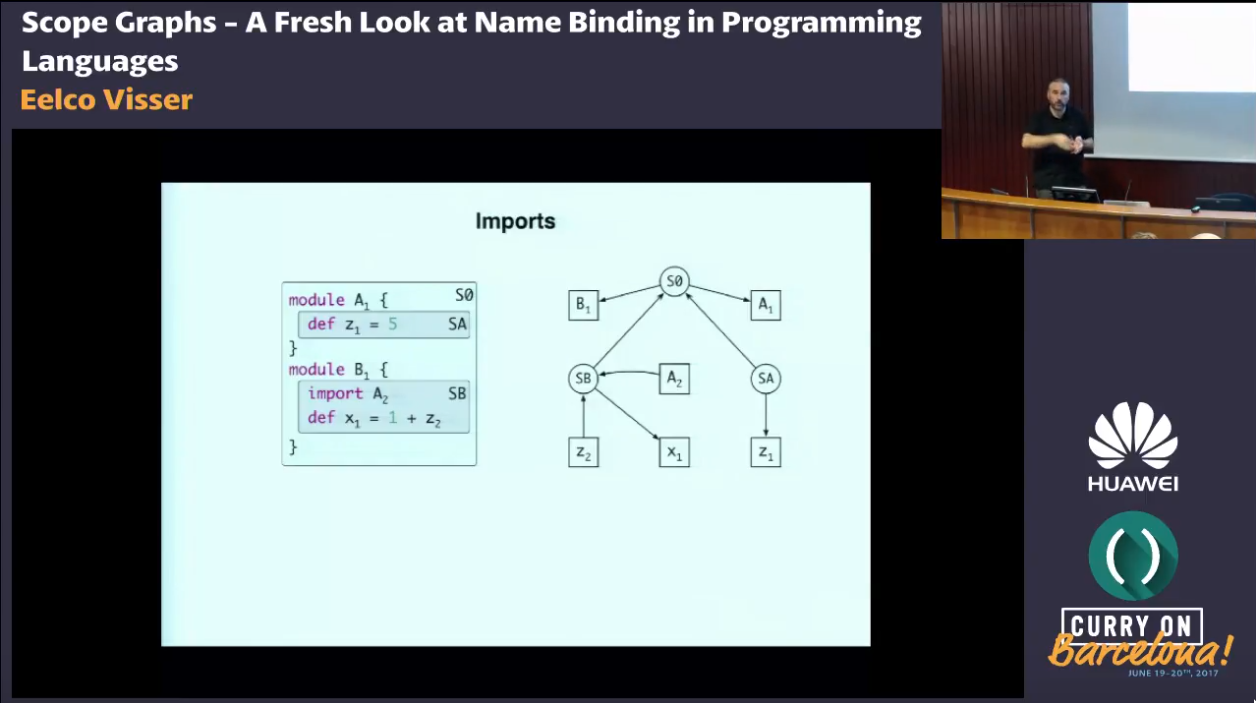
\includegraphics[width=60mm]{eelco-curry-on.png}
            }
        \end{center}
    \end{textblock*}
\end{frame}


\section{Code Navigation}

\begin{frame}
    \begin{textblock*}{160mm}(0mm,0mm)
        \picturecredit{Ivan Radic}{Close-up of a compass graffiti on the ground}{CC-BY-2.0}{https://flic.kr/p/2kGKMtM}
        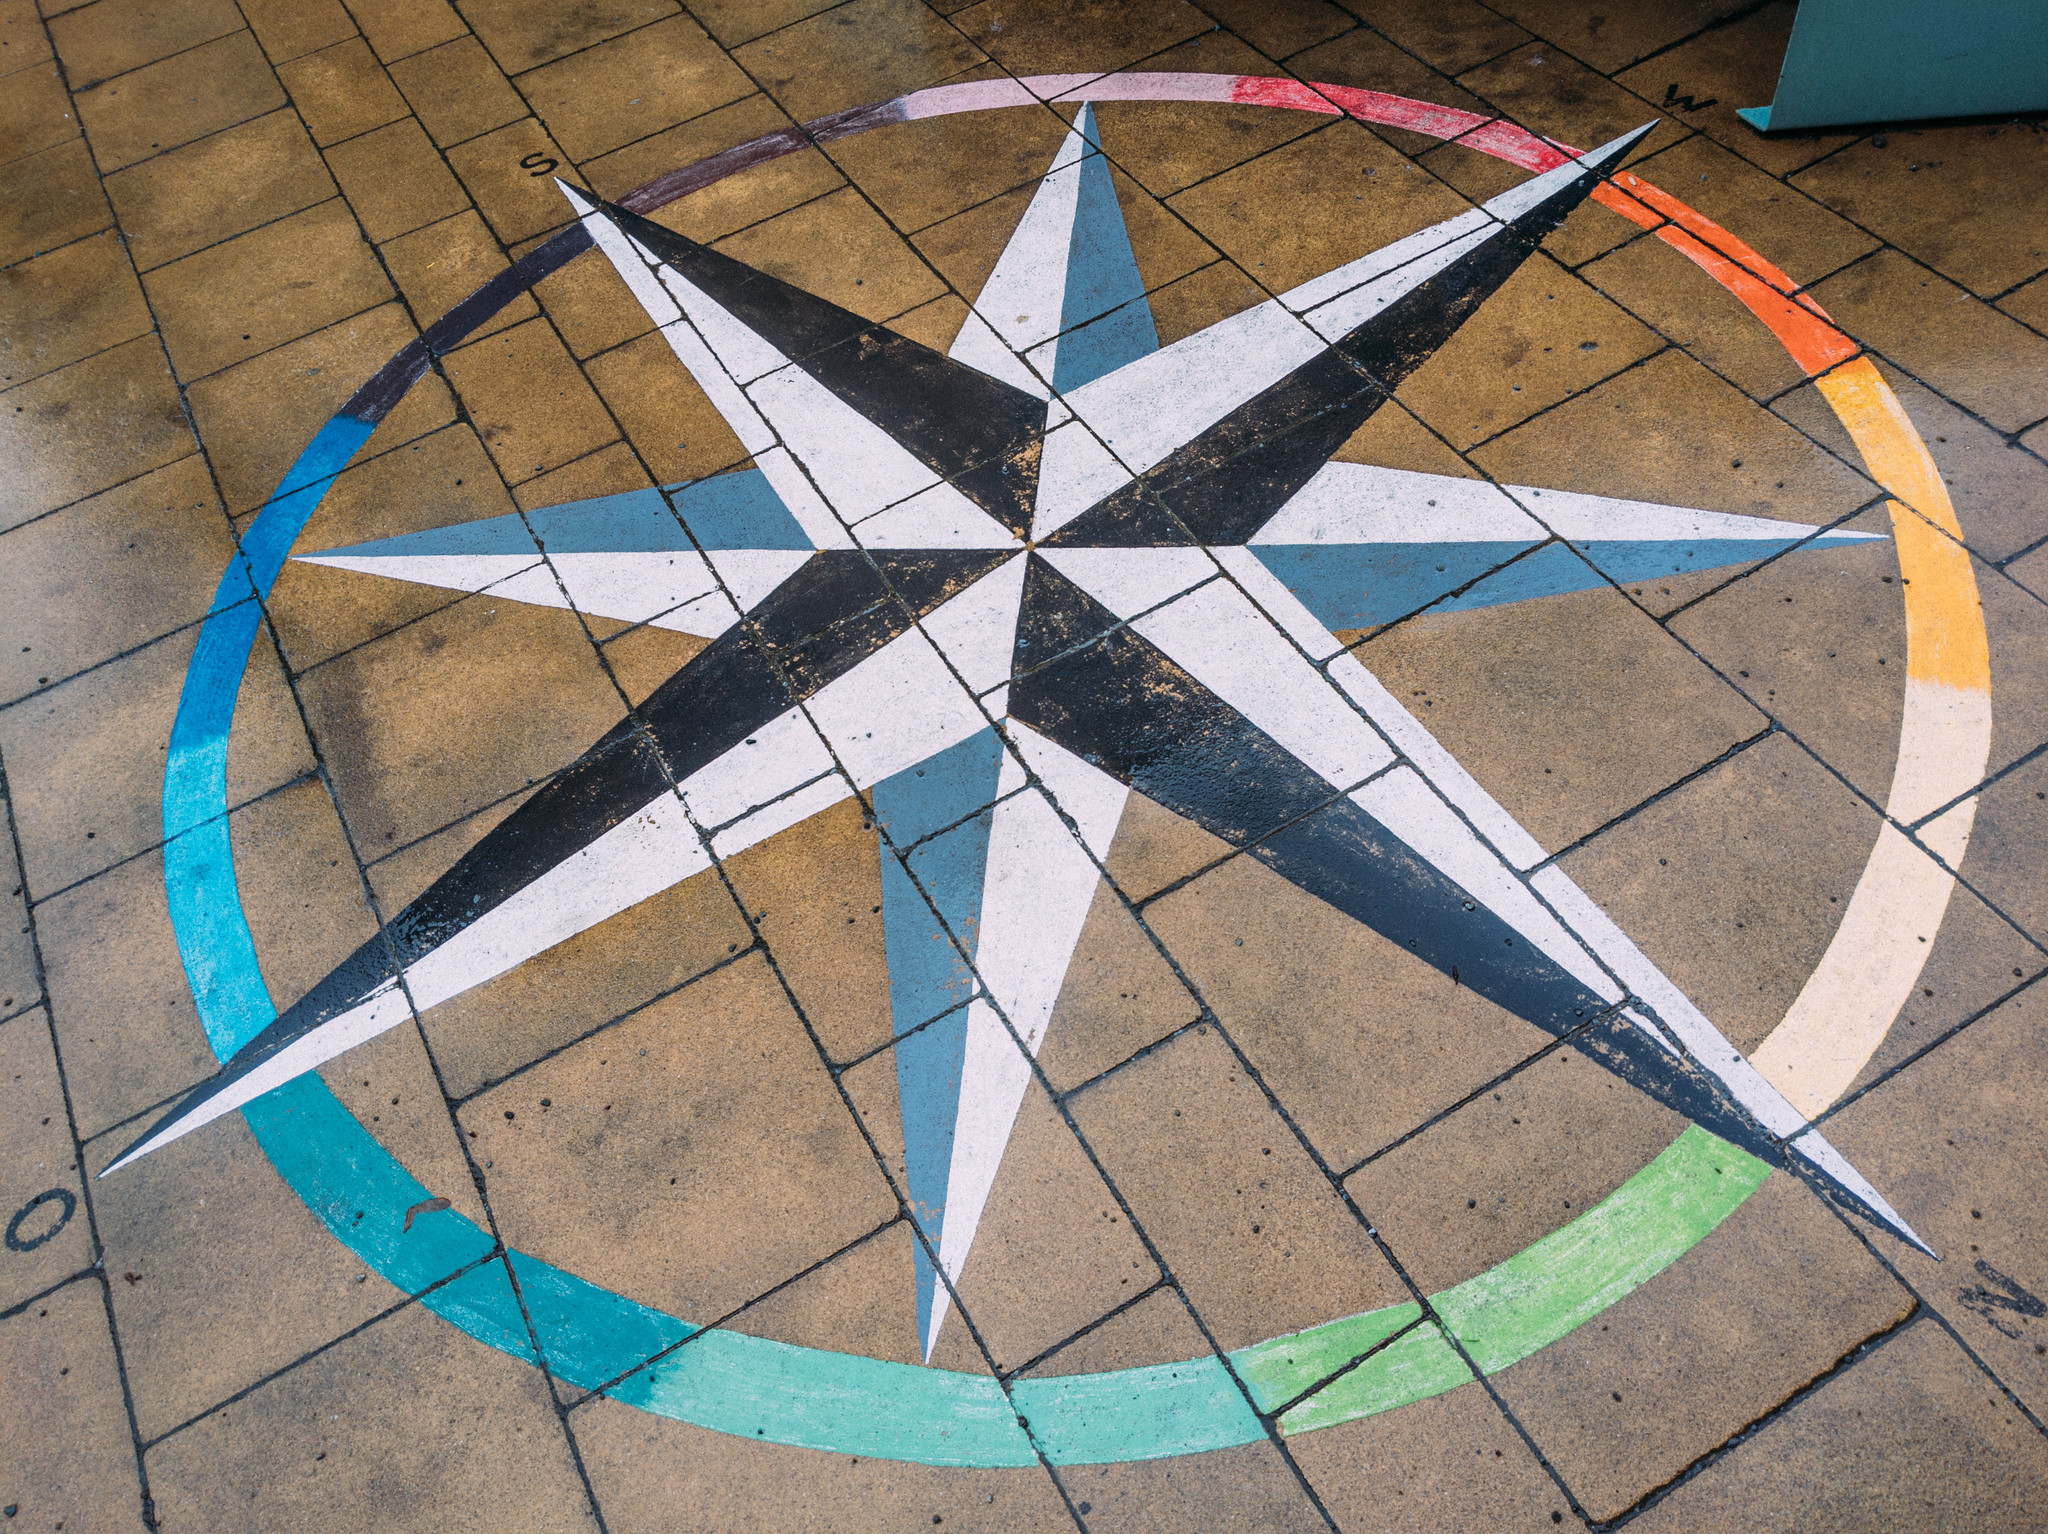
\includegraphics[width=160mm]{compass.jpg}
    \end{textblock*}
    \shadowedtitle{10mm}{10mm}{Code Navigation}
\end{frame}

% easy
\begin{frame}[fragile]
    \frametitle{Code Navigation}
    \uncover<2-3>{\highlightdef{def}}
    \uncover<2-3>{\highlightref{ref}}
    \begin{center}
    \begin{minipage}{9em}
    \begin{minted}[label=stove.py]{python}
        def bake():
            pass

        def ?\tikzmark{def_start}?broil?\tikzmark{def_end}?():
            pass

        def saute():
            pass

        ?\tikzmark{ref_start}?broil?\tikzmark{ref_end}?()
    \end{minted}
    \end{minipage}
    \end{center}
    \uncover<3>{\curvecodeline%
      {[yshift=8pt] pic cs:ref_end}%
      {+(25:2cm) and +(-45:1cm)}%
      {[yshift=-4pt] pic cs:def_end}%
    }%
\end{frame}


\section{Why is this hard?}

\begin{frame}
    \begin{textblock*}{160mm}(0mm,0mm)
        \picturecredit{Mustang Joe}{I swear...}{Public domain}{https://flic.kr/p/VSLwD6}
        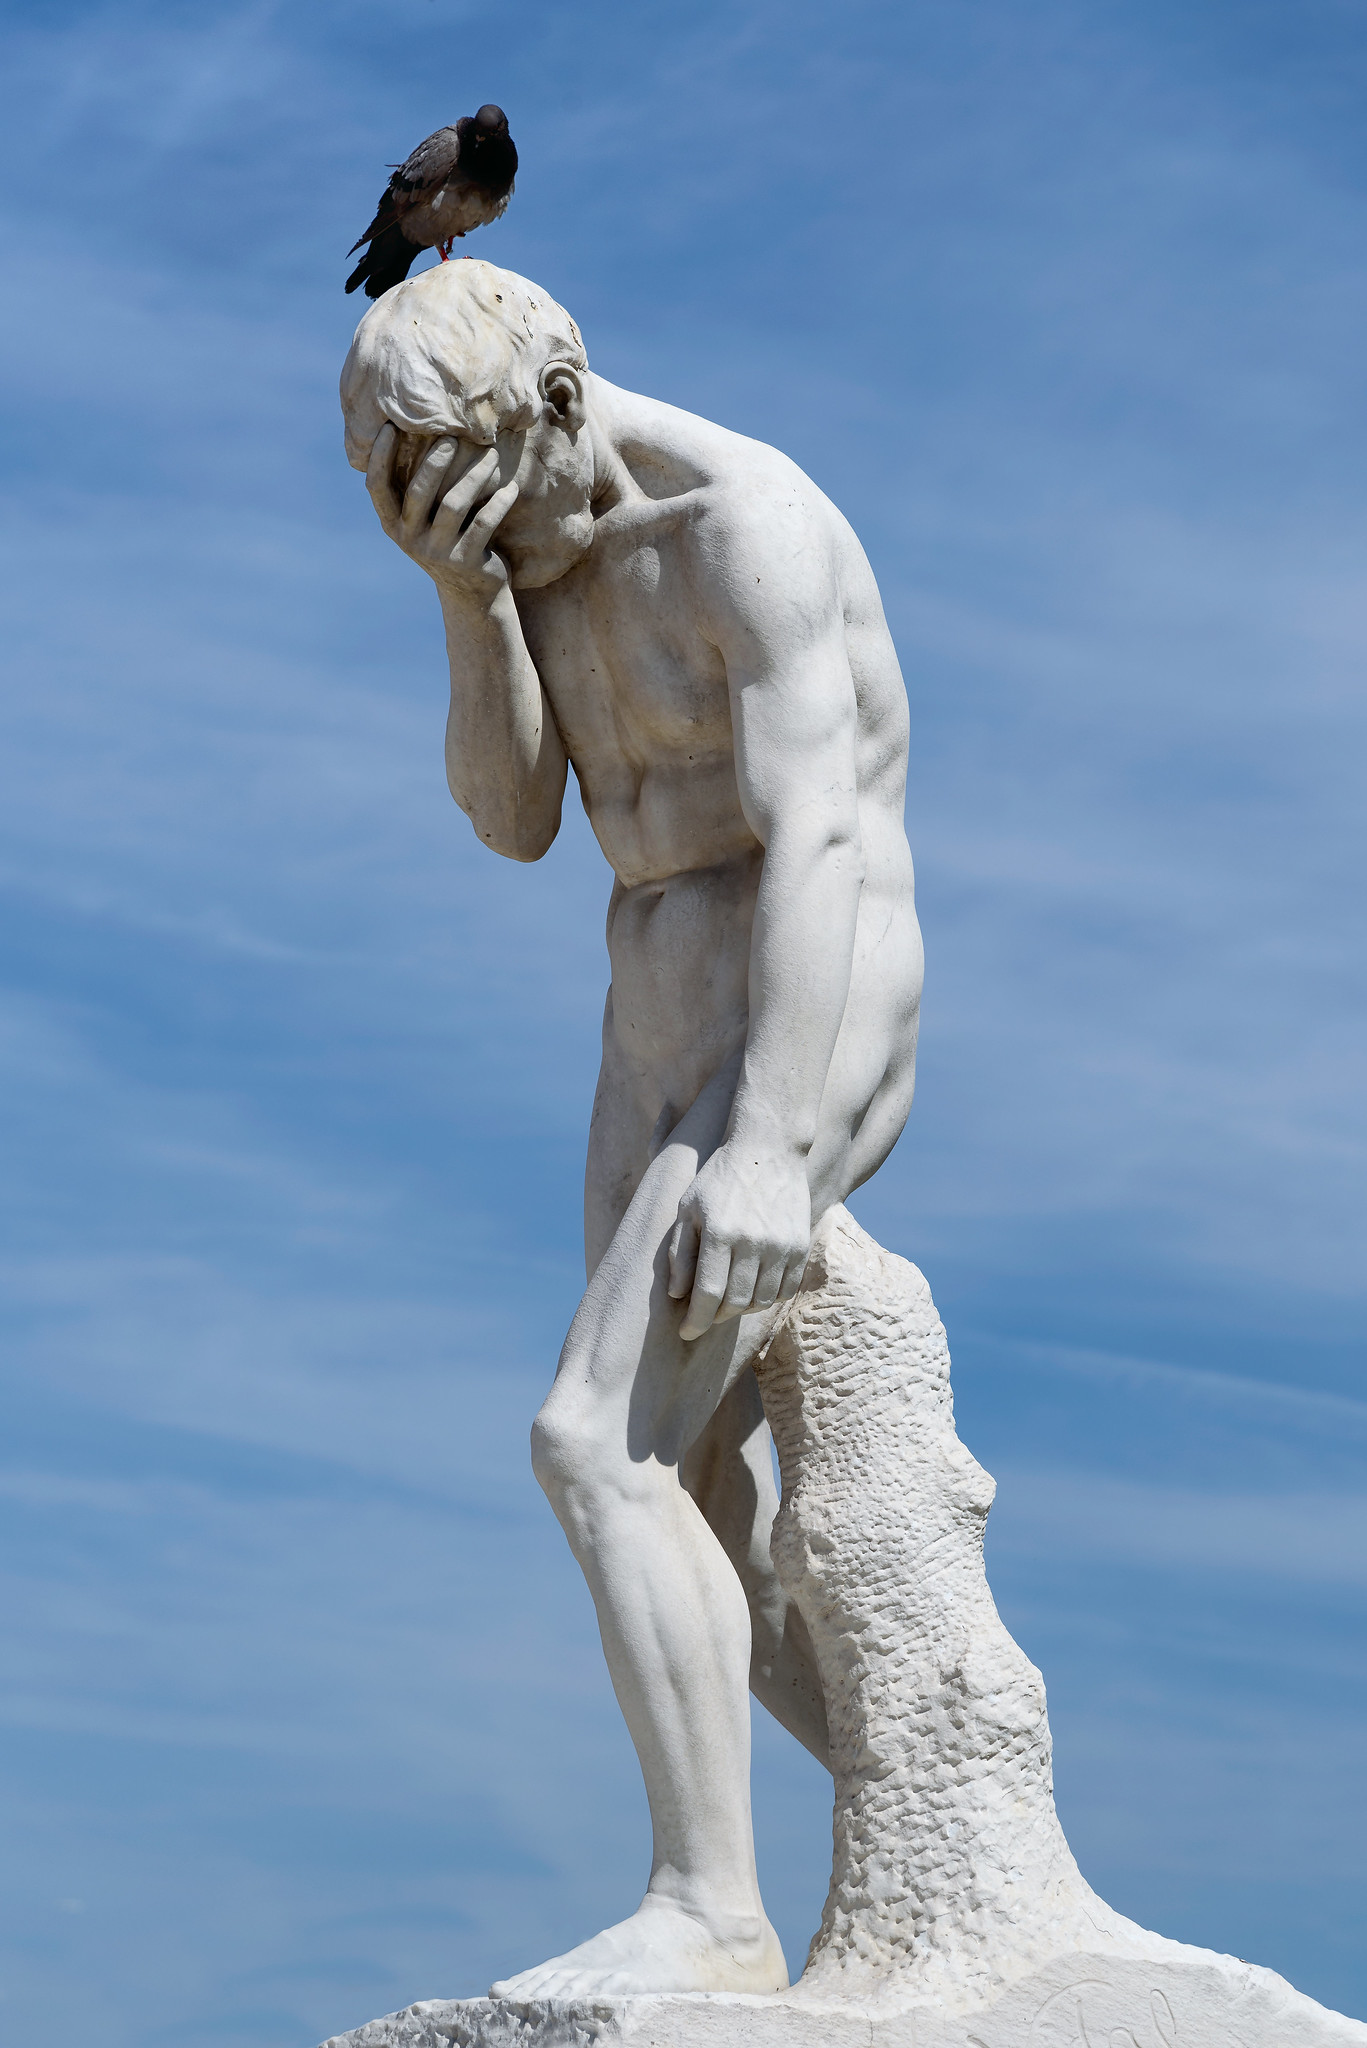
\includegraphics[width=160mm]{facepalm.jpg}
    \end{textblock*}
    \shadowedtitle{140mm - \titlewidth}{25mm}{Why is this hard?}
\end{frame}


% easy_shadowed
\begin{frame}[fragile]
    \frametitle{Why is this hard?}
    \uncover<2-3>{\highlightdef{def1}}
    \uncover<2-3>{\highlightdef{def2}}
    \uncover<2-3>{\highlightref{ref}}
    \begin{center}
    \begin{minipage}{9em}
    \begin{minted}[label=stove.py]{python}
        def ?\tikzmark{def1_start}?broil?\tikzmark{def1_end}?():
            pass

        def ?\tikzmark{def2_start}?broil?\tikzmark{def2_end}?():
            pass

        def saute():
            pass

        ?\tikzmark{ref_start}?broil?\tikzmark{ref_end}?()
    \end{minted}
    \end{minipage}
    \end{center}
    \uncover<3>{\curvecodeline%
      [dotted]%
      {[yshift=8pt] pic cs:ref_end}%
      {+(15:3cm) and +(-35:1cm)}%
      {[yshift=-4pt] pic cs:def1_end}%
    }%
    \uncover<3>{\curvecodeline%
      {[yshift=8pt] pic cs:ref_end}%
      {+(25:2cm) and +(-45:1cm)}%
      {[yshift=-4pt] pic cs:def2_end}%
    }%
\end{frame}


% easy_shadowed_rust
\begin{frame}[fragile]
    \frametitle{Why is this hard?}
    \uncover<2-3>{\highlightdef{def1}}
    \uncover<2-3>{\highlightdef{def2}}
    \uncover<2-3>{\highlightref{ref}}
    \begin{center}
    \begin{minipage}{9em}
    \begin{minted}[label=stove.rs]{rust}
        fn ?\tikzmark{def1_start}?broil?\tikzmark{def1_end}?() {}

        fn ?\tikzmark{def2_start}?broil?\tikzmark{def2_end}?() {}

        fn saute() {}

        fn main() {
          ?\tikzmark{ref_start}?broil?\tikzmark{ref_end}?();
        }
    \end{minted}
    \end{minipage}
    \end{center}
    \uncover<3>{%
        \tikz[remember picture]
          \node [overlay, text=red]
            at ([xshift=-2ex, yshift=0.5ex] pic cs:def2_end)
            {\textbf{\Huge X}};%
    }%
\end{frame}


% separate_files
\begin{frame}[fragile]
    \frametitle{Why is this hard?}
    \uncover<2-3>{\highlightdef{def}}
    \uncover<  3>{\highlightboth{import}}
    \uncover<2-3>{\highlightref{ref}}
    \begin{center}
    \begin{minipage}[t]{9em}
    \begin{minted}[label=stove.py]{python}
        def bake():
            pass

        def ?\tikzmark{def_start}?broil?\tikzmark{def_end}?():
            pass

        def saute():
            pass
    \end{minted}
    \end{minipage}
    \hspace{0.5em}
    \begin{minipage}[t]{11em}
    \begin{minted}[label=kitchen.py]{python}
        from stove import ?\tikzmark{import_start}?broil?\tikzmark{import_end}?

        ?\tikzmark{ref_start}?broil?\tikzmark{ref_end}?()
    \end{minted}
    \end{minipage}
    \end{center}
    \uncover<3>{\curvecodeline%
      [-]%
      {[yshift=10pt] pic cs:ref_end}%
      {+(45:1cm) and +(-155:1cm)}%
      {[yshift=-4pt] pic cs:import_start}%
    }
    \uncover<3>{\curvecodeline%
      {[xshift=12pt, yshift=10pt] pic cs:import_start}%
      {+(90:2cm) and +(75:2cm)}%
      {[xshift=-6pt, yshift=10pt] pic cs:def_end}%
    }
\end{frame}


% three_files
\begin{frame}[fragile]
    \uncover<2-3>{\highlightdef{def}}
    \uncover<  3>{\highlightboth{kitchen_import}}
    \uncover<  3>{\highlightboth{chef_import}}
    \uncover<2-3>{\highlightref{ref}}
    \frametitle{Why is this hard?}
    \begin{center}
    \begin{minipage}[t]{22.5em}
    \begin{center}
        
\includegraphics[height=2em]{icons/pan.png}
    \end{center}
    \vskip -1em
    \begin{minipage}[t]{7em}
    \begin{minted}[label=stove.py]{python}
        def bake():
            pass

        def ?\tikzmark{def_start}?broil?\tikzmark{def_end}?():
            pass

        def saute():
            pass
    \end{minted}
    \end{minipage}
    \hspace{0.5em}
    \begin{minipage}[t]{15em}
    \begin{minted}[label=kitchen.py]{python}
        from stove import ?\tikzmark{kitchen_import_start}?*?\tikzmark{kitchen_import_end}?
    \end{minted}
    \end{minipage}
    \end{minipage}
    \hspace{0.5em}
    \begin{minipage}[t]{12em}
    \vskip 8em
    \begin{center}
        
\includegraphics[height=2em]{icons/chef.png}
    \end{center}
    \begin{minted}[label=chef.py]{python}
        from kitchen import ?\tikzmark{chef_import_start}?broil?\tikzmark{chef_import_end}?

        ?\tikzmark{ref_start}?broil?\tikzmark{ref_end}?()
    \end{minted}
    \end{minipage}
    \end{center}
    \uncover<3>{\curvecodeline%
      [-]%
      {[yshift=10pt] pic cs:ref_end}%
      {+(45:1cm) and +(-155:1cm)}%
      {[yshift=-4pt] pic cs:chef_import_start}%
    }
    \uncover<3>{\curvecodeline%
      [-]%
      {[xshift=10pt, yshift=10pt] pic cs:chef_import_start}%
      {+(90:5cm) and +(75:2cm)}%
      {[xshift=4pt, yshift=10pt] pic cs:kitchen_import_start}%
    }
    \uncover<3>{\curvecodeline%
      {[xshift=1pt, yshift=-4pt] pic cs:kitchen_import_start}%
      {+(-105:1cm) and +(75:1cm)}%
      {[xshift=-6pt, yshift=10pt] pic cs:def_end}%
    }
\end{frame}


% three_files_updated
\begin{frame}[fragile]
    \frametitle{Why is this hard?}
    \uncover<2-3>{\highlightdef{def1}}
    \uncover<2-3>{\highlightdef{def2}}
    \uncover<  3>{\highlightboth{import}}
    \uncover<2-3>{\highlightref{ref}}
    \begin{center}
    \begin{minipage}[t]{22.5em}
    \begin{center}
        
\includegraphics[height=2em]{icons/pan.png}
    \end{center}
    \vskip -1em
    \begin{minipage}[t]{7em}
    \begin{minted}[label=stove.py]{python}
        def bake():
            pass

        def ?\tikzmark{def1_start}?broil?\tikzmark{def1_end}?():
            pass

        def saute():
            pass
    \end{minted}
    \end{minipage}
    \hspace{0.5em}
    \begin{minipage}[t]{15em}
    \begin{minted}[label=kitchen.py]{python}
        from stove import *

        def ?\tikzmark{def2_start}?broil?\tikzmark{def2_end}?():
            print("We're broiling!")
            import stove
            return stove.broil()
    \end{minted}
    \end{minipage}
    \end{minipage}
    \hspace{0.5em}
    \begin{minipage}[t]{12em}
    \vskip 8em
    \begin{center}
        
\includegraphics[height=2em]{icons/chef.png}
    \end{center}
    \begin{minted}[label=chef.py]{python}
        from kitchen import ?\tikzmark{import_start}?broil?\tikzmark{import_end}?

        ?\tikzmark{ref_start}?broil?\tikzmark{ref_end}?()
    \end{minted}
    \end{minipage}
    \end{center}
    \uncover<3>{\curvecodeline%
      [-]%
      {[yshift=10pt] pic cs:ref_end}%
      {+(45:1cm) and +(-155:1cm)}%
      {[yshift=-4pt] pic cs:import_start}%
    }
    \uncover<3>{\curvecodeline%
      {[xshift=10pt, yshift=10pt] pic cs:import_start}%
      {+(90:5cm) and +(75:2cm)}%
      {[xshift=-6pt, yshift=10pt] pic cs:def2_end}%
    }
\end{frame}


% python_class
\begin{frame}[fragile]
    \frametitle{Why is this hard?}
    \begin{center}
    \uncover<2- >{\highlightdef{def}}%
    \uncover<2- >{\highlightref{ref}}%
    \begin{minipage}[t]{25.5em}
    \begin{center}
        
\includegraphics[height=2em]{icons/pan.png}
    \end{center}
    \vskip -1em
    \begin{minipage}[t]{10em}
    \begin{minted}[label=stove.py]{python}
        class?\tikzmark{class}? Stove?\tikzmark{class_def}?(object):
            def bake(self):
                pass

            def ?\tikzmark{def_start}?broil?\tikzmark{def_end}?(self):
                pass

            def saute(self):
                pass
    \end{minted}
    \end{minipage}
    \hspace{0.5em}
    \begin{minipage}[t]{15em}
    \begin{minted}[label=kitchen.py]{python}
        from stove import ?\tikzmark{kitchen_import}?*
    \end{minted}
    \end{minipage}
    \end{minipage}
    \hspace{-5.5em}
    \begin{minipage}[t]{12em}
    \vskip 6em
    \begin{center}
        
\includegraphics[height=2em]{icons/chef.png}
    \end{center}
    \begin{minted}[label=chef.py]{python}
        from kitchen import ?\tikzmark{chef_import}?Stove

        stove?\tikzmark{instance_def}? = Stove?\tikzmark{class_ref}?()
        stove?\tikzmark{instance_ref}?.?\tikzmark{ref_start}?broil?\tikzmark{ref_end}?()
    \end{minted}
    \end{minipage}
    \end{center}
    \uncover<3- >{\curvecodeline%
      [-]%
      {[xshift=-10pt, yshift=-3pt] pic cs:ref_end}%
      {+(-135:0.2cm) and +(-45:0.2cm)}%
      {[xshift=-10pt, yshift=-3pt] pic cs:instance_ref}%
    }
    \uncover<3- >{\curvecodeline%
      [-]%
      {[xshift=-23pt, yshift=2pt] pic cs:instance_ref}%
      {+(180:0.2cm) and +(180:0.2cm)}%
      {[xshift=-23pt, yshift=2pt] pic cs:instance_def}%
    }
    \uncover<3- >{\curvecodeline%
      [-]%
      {[xshift=-10pt, yshift=8pt] pic cs:instance_def}%
      {+(65:0.3cm) and +(115:0.3cm)}%
      {[xshift=-10pt, yshift=8pt] pic cs:class_ref}%
    }
    \uncover<3- >{\curvecodeline%
      [-]%
      {[xshift=-4pt, yshift=-3pt] pic cs:class_ref}%
      {+(-35:0.5cm) and +(-90:1cm)}%
      {[xshift=10pt, yshift=-3pt] pic cs:chef_import}%
    }
    \uncover<3- >{\curvecodeline%
      [-]%
      {[xshift=10pt, yshift=10pt] pic cs:chef_import}%
      {+(90:3cm) and +(-90:1cm)}%
      {[xshift=2pt, yshift=-3pt] pic cs:kitchen_import}%
    }
    \uncover<3- >{\curvecodeline%
      [-]%
      {[xshift=2pt, yshift=10pt] pic cs:kitchen_import}%
      {+(90:2cm) and +(90:2cm)}%
      {[xshift=-10pt, yshift=8pt] pic cs:class_def}%
    }
    \uncover<3- >{\curvecodeline%
      [-]%
      {[xshift=-6pt, yshift=-2pt] pic cs:class_def}%
      {+(-45:2cm) and +(90:2cm)}%
      {[xshift=4pt, yshift=10pt] pic cs:class_ref}%
    }
    \uncover<3- >{\curvecodeline%
      [-]%
      {[xshift=4pt, yshift=-3pt] pic cs:class_ref}%
      {+(-90:2.5cm) and +(-90:6.5cm)}%
      {[xshift=-10pt, yshift=-2pt] pic cs:class}%
    }
    \uncover<3- >{\curvecodeline%
      {[xshift=-10pt, yshift=8pt] pic cs:class}%
      {+(75:1cm) and +(115:1cm)}%
      {[xshift=-10pt, yshift=6pt] pic cs:def_end}%
    }
\end{frame}


% dataflow
\begin{frame}[fragile]
    \frametitle{Why is this hard?}
    \uncover<2-3>{\highlightdef{def}}
    \uncover<2-3>{\highlightref{ref}}
    \begin{center}
    \begin{minipage}[t]{9em}
    \begin{minted}[label=dataflow.py]{python}
        def ?\tikzmark{passthrough_def_start}?passthrough(?\tikzmark{x_def_start}?x?\tikzmark{x_def_end}?):
            return ?\tikzmark{x_ref_start}?x?\tikzmark{x_ref_end}?
    \end{minted}
    \end{minipage}
    \hspace{0.5em}
    \begin{minipage}[t]{15em}
    \begin{minted}[label=a.py]{python}
        from dataflow import ?\tikzmark{passthrough_import_start}?passthrough?\tikzmark{passthrough_import_end}?

        class ?\tikzmark{A_def_start}?A?\tikzmark{A_def_end}?:
            ?\tikzmark{def_start}?one?\tikzmark{def_end}? = 1

        ?\tikzmark{passthrough_ref_start}?passthrough?\tikzmark{passthrough_ref_end}?(?\tikzmark{A_ref_start}?A?\tikzmark{A_ref_end}?).?\tikzmark{ref_start}?one?\tikzmark{ref_end}?
    \end{minted}
    \end{minipage}
    \end{center}
    \uncover<3>{\curvecodeline%
      [-]%
      {[yshift=-4pt] pic cs:ref_start}%
      {+(-135:0.5cm) and +(-75:0.5cm)}%
      {[xshift=15pt, yshift=-4pt] pic cs:passthrough_ref_start}%
    }%
    \uncover<3>{\curvecodeline%
      [-]%
      {[xshift=15pt, yshift=8pt] pic cs:passthrough_ref_start}%
      {+(75:1cm) and +(-90:1cm)}%
      {[xshift=15pt, yshift=-4pt] pic cs:passthrough_import_start}%
    }%
    \uncover<3>{\curvecodeline%
      [-]%
      {[xshift=15pt, yshift=8pt] pic cs:passthrough_import_start}%
      {+(90:1cm) and +(90:1cm)}%
      {[xshift=13pt, yshift=8pt] pic cs:passthrough_def_start}%
    }%
    \uncover<3>{\curvecodeline%
      [-]%
      {[xshift=15pt, yshift=-2pt] pic cs:passthrough_def_start}%
      {+(-45:0.25cm) and +(180:0.25cm)}%
      {[xshift=-2pt, yshift=3pt] pic cs:x_ref_start}%
    }%
    \uncover<3>{\curvecodeline%
      [-]%
      {[xshift=2pt, yshift=3pt] pic cs:x_ref_end}%
      {+(0:0.25cm) and +(180:0.25cm)}%
      {[xshift=-2pt, yshift=2pt] pic cs:x_def_start}%
    }%
    \uncover<3>{\curvecodeline%
      [-]%
      {[xshift=2pt, yshift=2pt] pic cs:x_def_end}%
      {+(0:4cm) and +(0:1cm)}%
      {[xshift=2pt, yshift=4pt] pic cs:A_ref_end}%
    }%
    \uncover<3>{\curvecodeline%
      [-]%
      {[xshift=-2pt, yshift=4pt] pic cs:A_ref_start}%
      {+(175:0.5cm) and +(-85:0.5cm)}%
      {[xshift=-1pt, yshift=-4pt] pic cs:A_def_end}%
    }%
    \uncover<3>{\curvecodeline%
      {[xshift=1pt, yshift=8pt] pic cs:A_def_start}%
      {+(105:0.5cm) and +(90:0.5cm)}%
      {[xshift=4pt, yshift=8pt] pic cs:def_start}%
    }%
\end{frame}


\begin{frame}
    \begin{textblock*}{160mm}(0mm,0mm)
        \picturecredit{Marco Verch}{Close-up, a piece of yellow cake with red currant berries}{CC-BY-2.0}{https://flic.kr/p/2jikJsQ}
        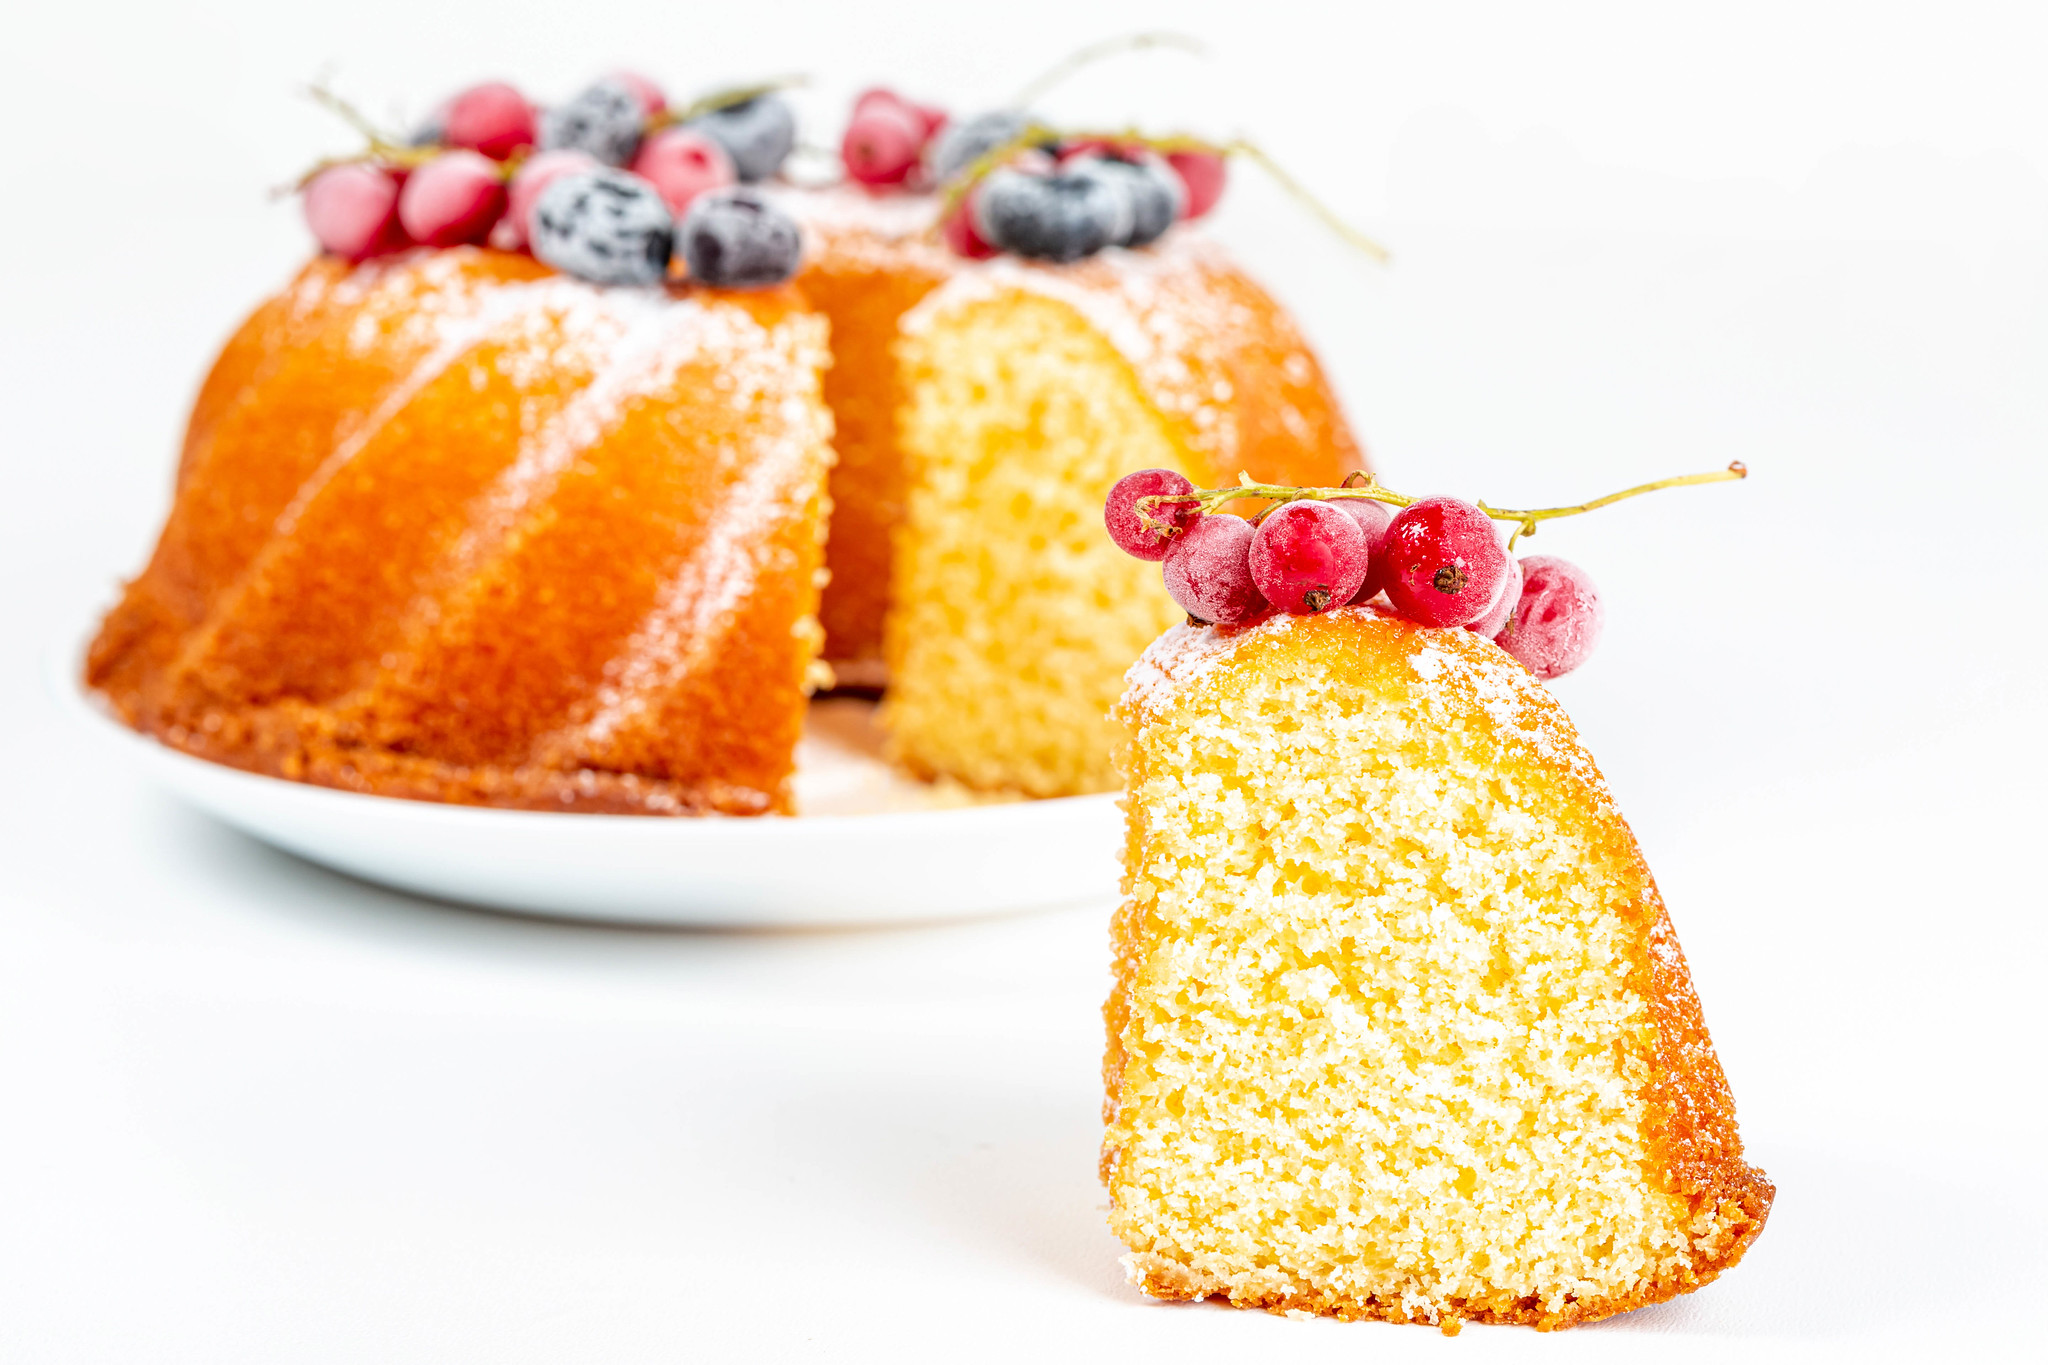
\includegraphics[width=160mm]{cake.jpg}
    \end{textblock*}
    \flattitle{10mm}{80mm}{Oh is that all?}
\end{frame}


\begin{frame}
    \frametitle{Zero configuration}
    \begin{center}
        We don't want to have to ask the package \\ owner how to collect the data
        we need.
    \end{center}
    \begin{center}
        Or ask them to configure a job to produce that data.
    \end{center}
    \begin{center}
        It should \strong{Just Work}.
    \end{center}
\end{frame}


\begin{frame}
    %\begin{textblock*}{80mm}(80mm,0mm)
    %    \picturecredit{Mark Gunn}{This just tern'ed into a swarm!}{CC-BY-2.0}{https://flic.kr/p/P11JH1}
    %    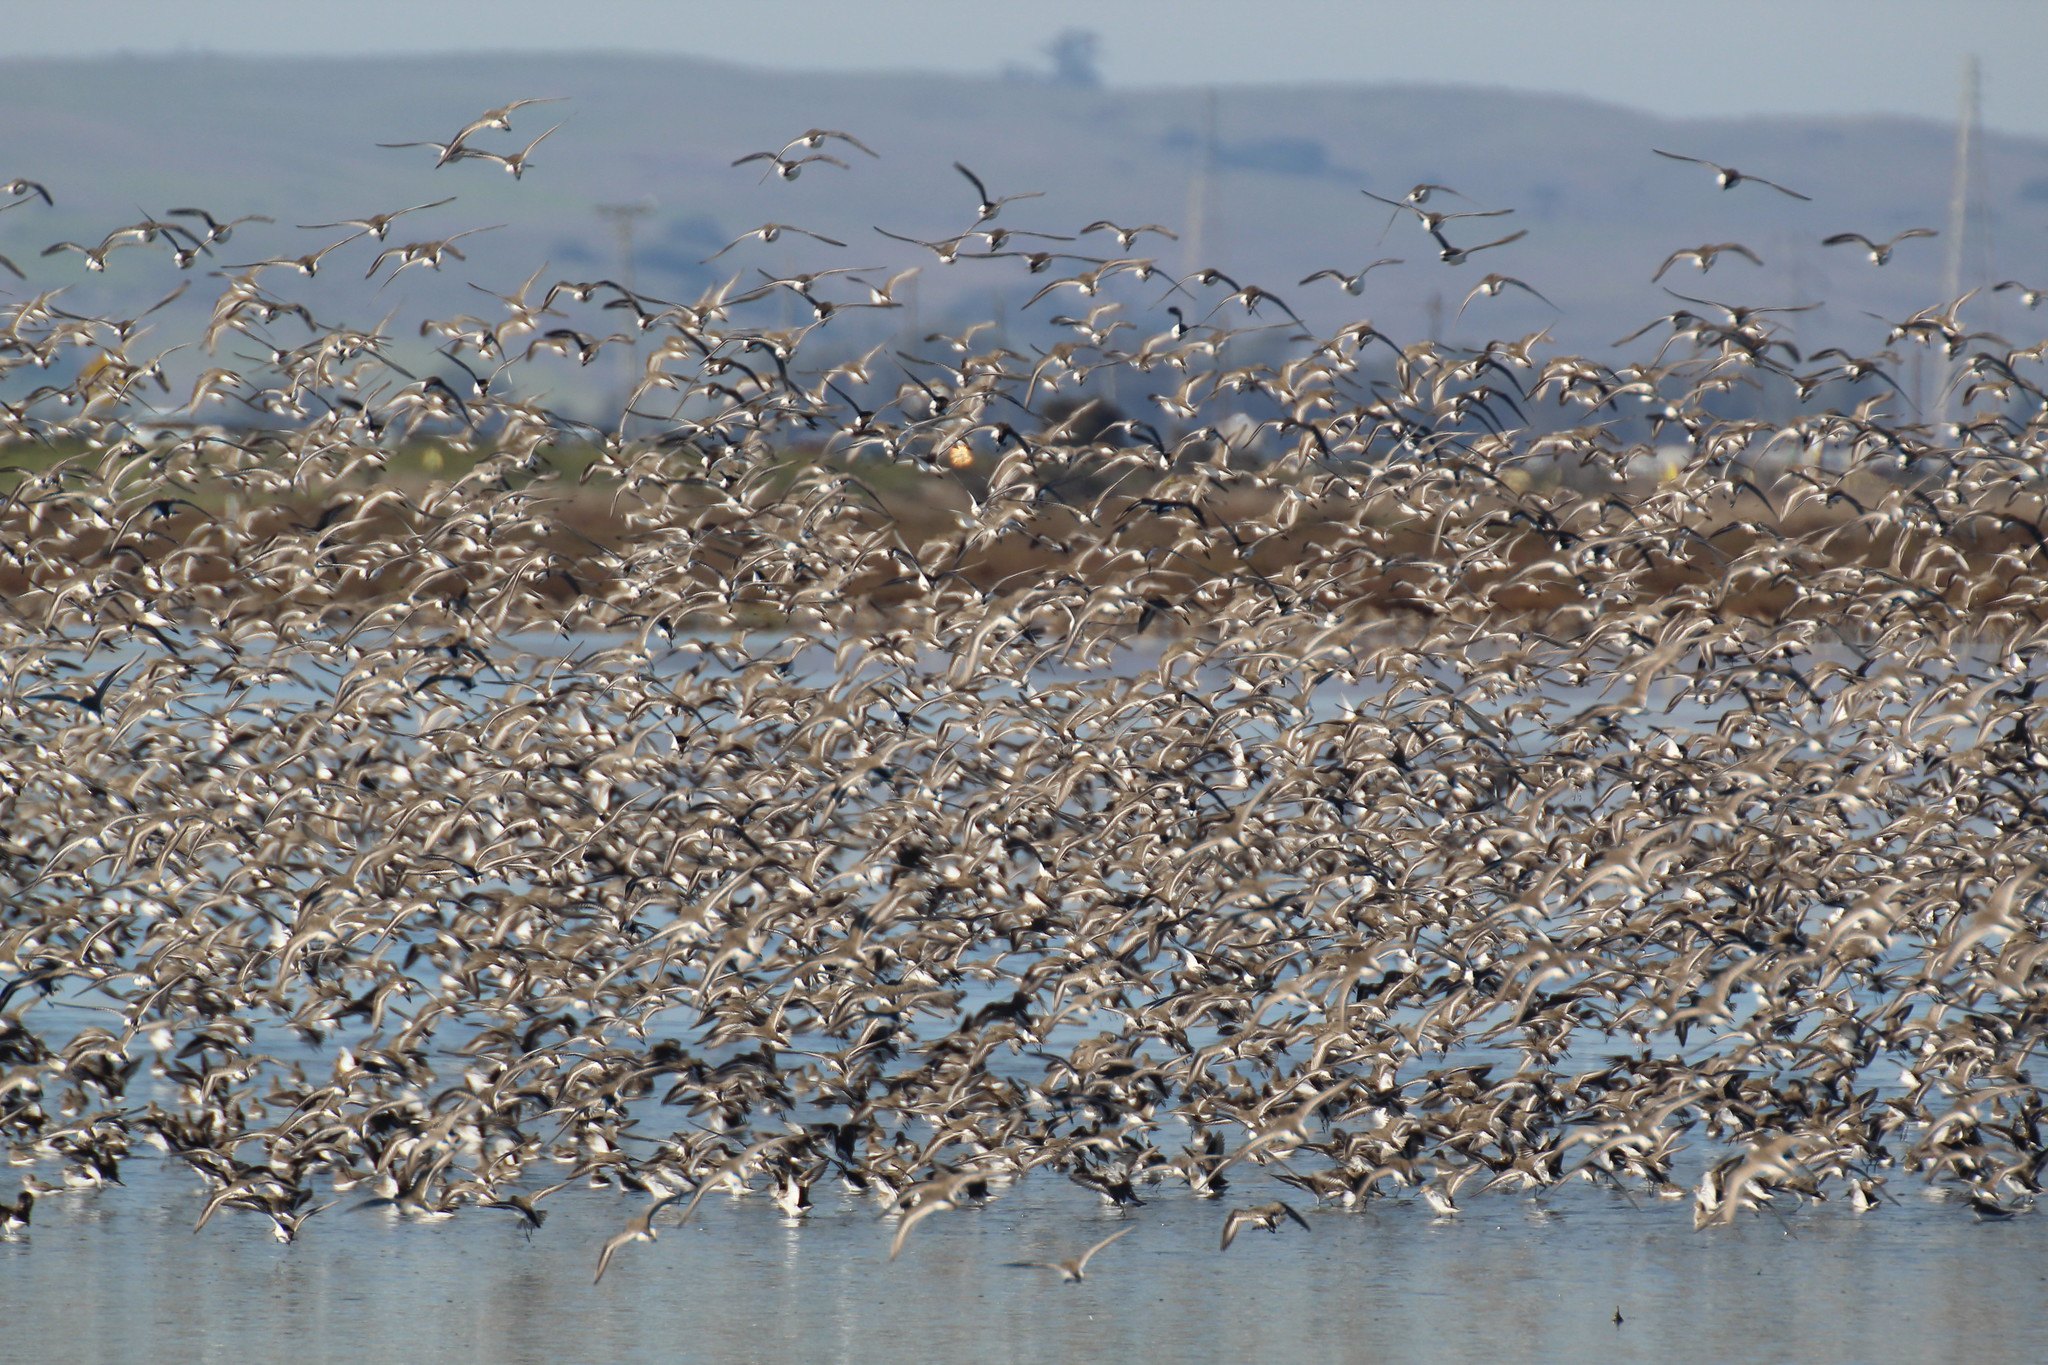
\includegraphics[width=160mm]{terns.jpg}
    %\end{textblock*}
    \begin{textblock*}{80mm}(80mm,0mm)
        \picturecredit{Joseph Gage}{Massive goose gaggle}{CC-BY-SA-2.0}{https://flic.kr/p/2kJfaCt}
        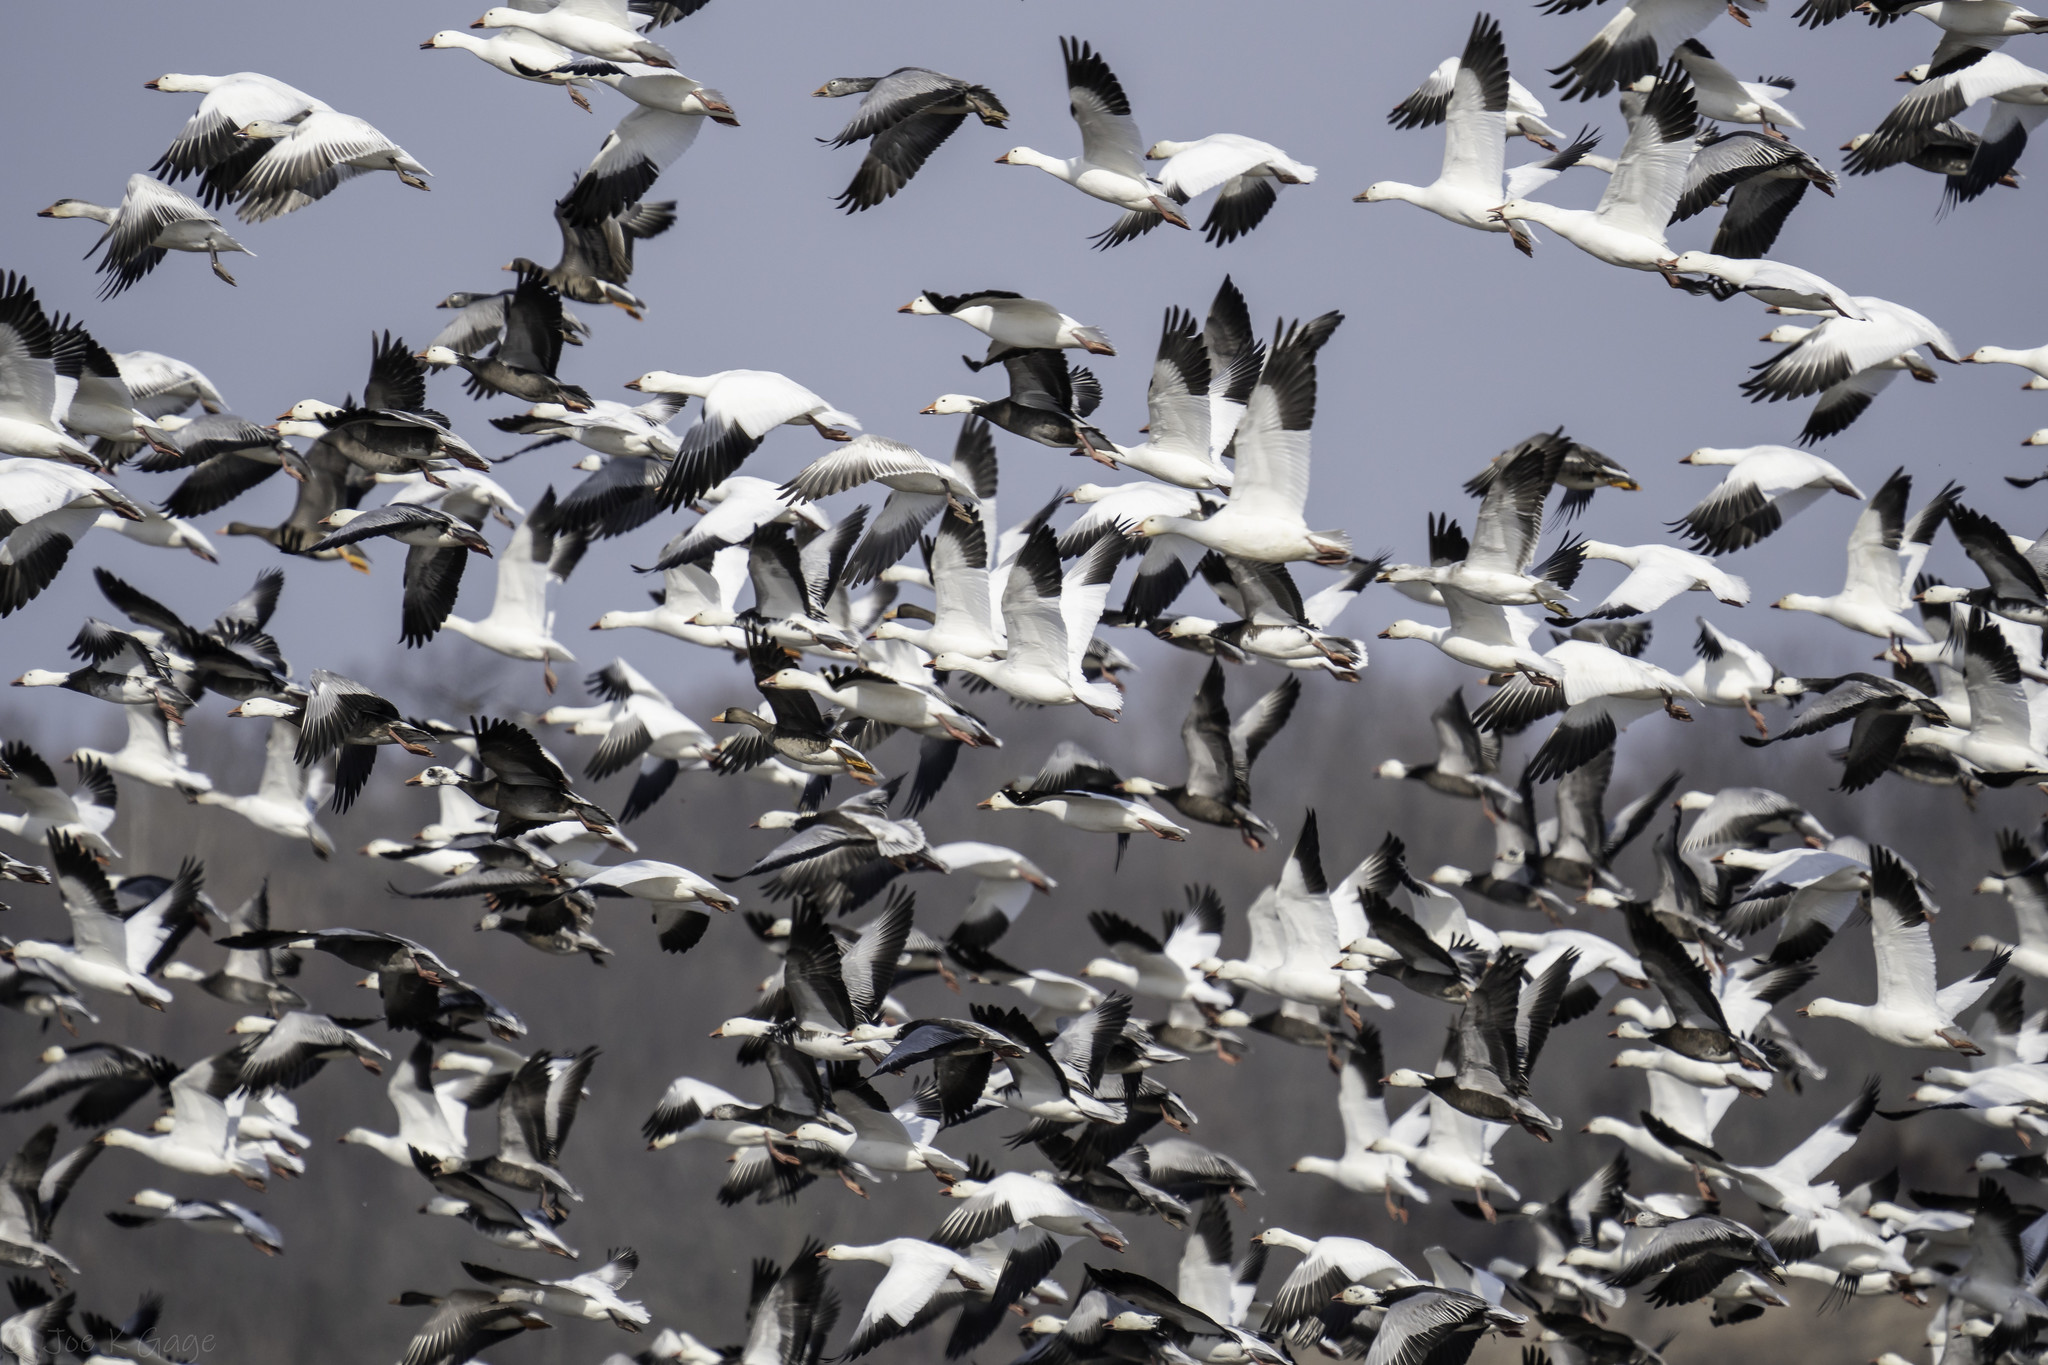
\includegraphics[width=160mm]{geese.jpg}
    \end{textblock*}

    \frametitle{SCALE}
    200 million repositories and counting
    \vskip 1em
    2 billion contributions \\
    in the last 12 months
    \vskip 1em
    500 programming languages
\end{frame}


\begin{frame}[t]
    \frametitle{When do we do the work?}
    \vskip 2em
    \begin{tikzpicture}
        \node (bar) at(0,0) [
            rectangle, anchor=west,
            minimum width=\columnwidth, minimum height=1cm,
            draw=black, thin,
            fill=gray!20,
        ] {};

        \node at(bar.west) [
            rectangle, anchor=west, inner xsep=2ex,
            text height=1.5ex, text depth=0.25ex,
            text=black,
        ] {Index};
        \node at(bar.east) [
            rectangle, anchor=east, inner xsep=2ex,
            text height=1.5ex, text depth=0.25ex,
            text=black,
        ] {Query};
    \end{tikzpicture}
\end{frame}


\begin{frame}[t]
    \frametitle{When do we do the work?}
    \vskip 2em
    \begin{tikzpicture}
        \node (bar) at(0,0) [
            rectangle, anchor=west,
            minimum width=\columnwidth, minimum height=1cm,
            draw=black, thin,
            fill=gray!20,
        ] {};

        \node (query) at(bar.east) [
            rectangle, anchor=east,
            minimum width=0.8\columnwidth, minimum height=1cm,
            draw=black, thin,
            fill=blue!20,
        ] {};

        \node at (query.center) [overlay, text=red] {\scalebox{2}{\textbf{\Huge X}}};%

        \node at(bar.west) [
            rectangle, anchor=west, inner xsep=2ex,
            text height=1.5ex, text depth=0.25ex,
            text=black,
        ] {Index};
        \node at(bar.east) [
            rectangle, anchor=east, inner xsep=2ex,
            text height=1.5ex, text depth=0.25ex,
            text=black,
        ] {Query};
    \end{tikzpicture}

    \begin{center}
        This is an interactive feature, so we can't do too much work at query
        time.
    \end{center}
    \begin{center}
        Goal: < 100ms
    \end{center}
\end{frame}


\begin{frame}[t]
    \frametitle{When do we do the work?}
    \vskip 2em
    \begin{tikzpicture}
        \node (bar) at(0,0) [
            rectangle, anchor=west,
            minimum width=\columnwidth, minimum height=1cm,
            draw=black, thin,
            fill=gray!20,
        ] {};

        \node (index) at(bar.west) [
            rectangle, anchor=west,
            minimum width=0.8\columnwidth, minimum height=1cm,
            draw=black, thin,
            fill=yellow!20,
        ] {};

        \node at (index.center) [overlay, text=red] {\scalebox{2}{\textbf{\Huge X}}};%

        \node at(bar.west) [
            rectangle, anchor=west, inner xsep=2ex,
            text height=1.5ex, text depth=0.25ex,
            text=black,
        ] {Index};
        \node at(bar.east) [
            rectangle, anchor=east, inner xsep=2ex,
            text height=1.5ex, text depth=0.25ex,
            text=black,
        ] {Query};
    \end{tikzpicture}

    \begin{center}
        Because of our scale, we can't doo too much work at index time, either!

        (Compute and storage costs are too high, work is wasted, etc.)
    \end{center}
\end{frame}


\begin{frame}[t]
    \frametitle{When do we do the work?}
    \vskip 2em
    \begin{tikzpicture}
        \node (bar) at(0,0) [
            rectangle, anchor=west,
            minimum width=\columnwidth, minimum height=1cm,
            draw=black, thin,
            fill=gray!20,
        ] {};

        \node at(bar.west) [
            rectangle, anchor=west,
            minimum width=0.5\columnwidth, minimum height=1cm,
            draw=black, thin,
            fill=yellow!20,
        ] {};
        \node at(bar.east) [
            rectangle, anchor=east,
            minimum width=0.5\columnwidth, minimum height=1cm,
            draw=black, thin,
            fill=blue!20,
        ] {};

        \node at(bar.west) [
            rectangle, anchor=west, inner xsep=2ex,
            text height=1.5ex, text depth=0.25ex,
            text=black,
        ] {Index};
        \node at(bar.east) [
            rectangle, anchor=east, inner xsep=2ex,
            text height=1.5ex, text depth=0.25ex,
            text=black,
        ] {Query};
    \end{tikzpicture}

    \begin{center}
        We want to strike a balance.
    \end{center}

    \begin{center}
        Precalculate as much as we can.

        Minimize the amount of \strong{duplicated} work.

        Defer \strong{some} work until query time to make that happen.
    \end{center}
\end{frame}


\begin{frame}
    \frametitle{Why is this hard?}
    \begin{itemize}
        \item Different languages have different name binding rules.
        \item Some of those rules can be quite complex.
        \item The result might depend on intermediate files.
        \item We don't want to require manual per-repo configuration.
        \item We need to balance work between index time vs query time.
    \end{itemize}
\end{frame}


\section{Incremental results}

\begin{frame}
    \begin{textblock*}{160mm}(0mm,-15mm)
        \picturecredit{Katja Schulz}{Inchworm}{CC-BY-2.0}{https://flic.kr/p/PJMP4w}
        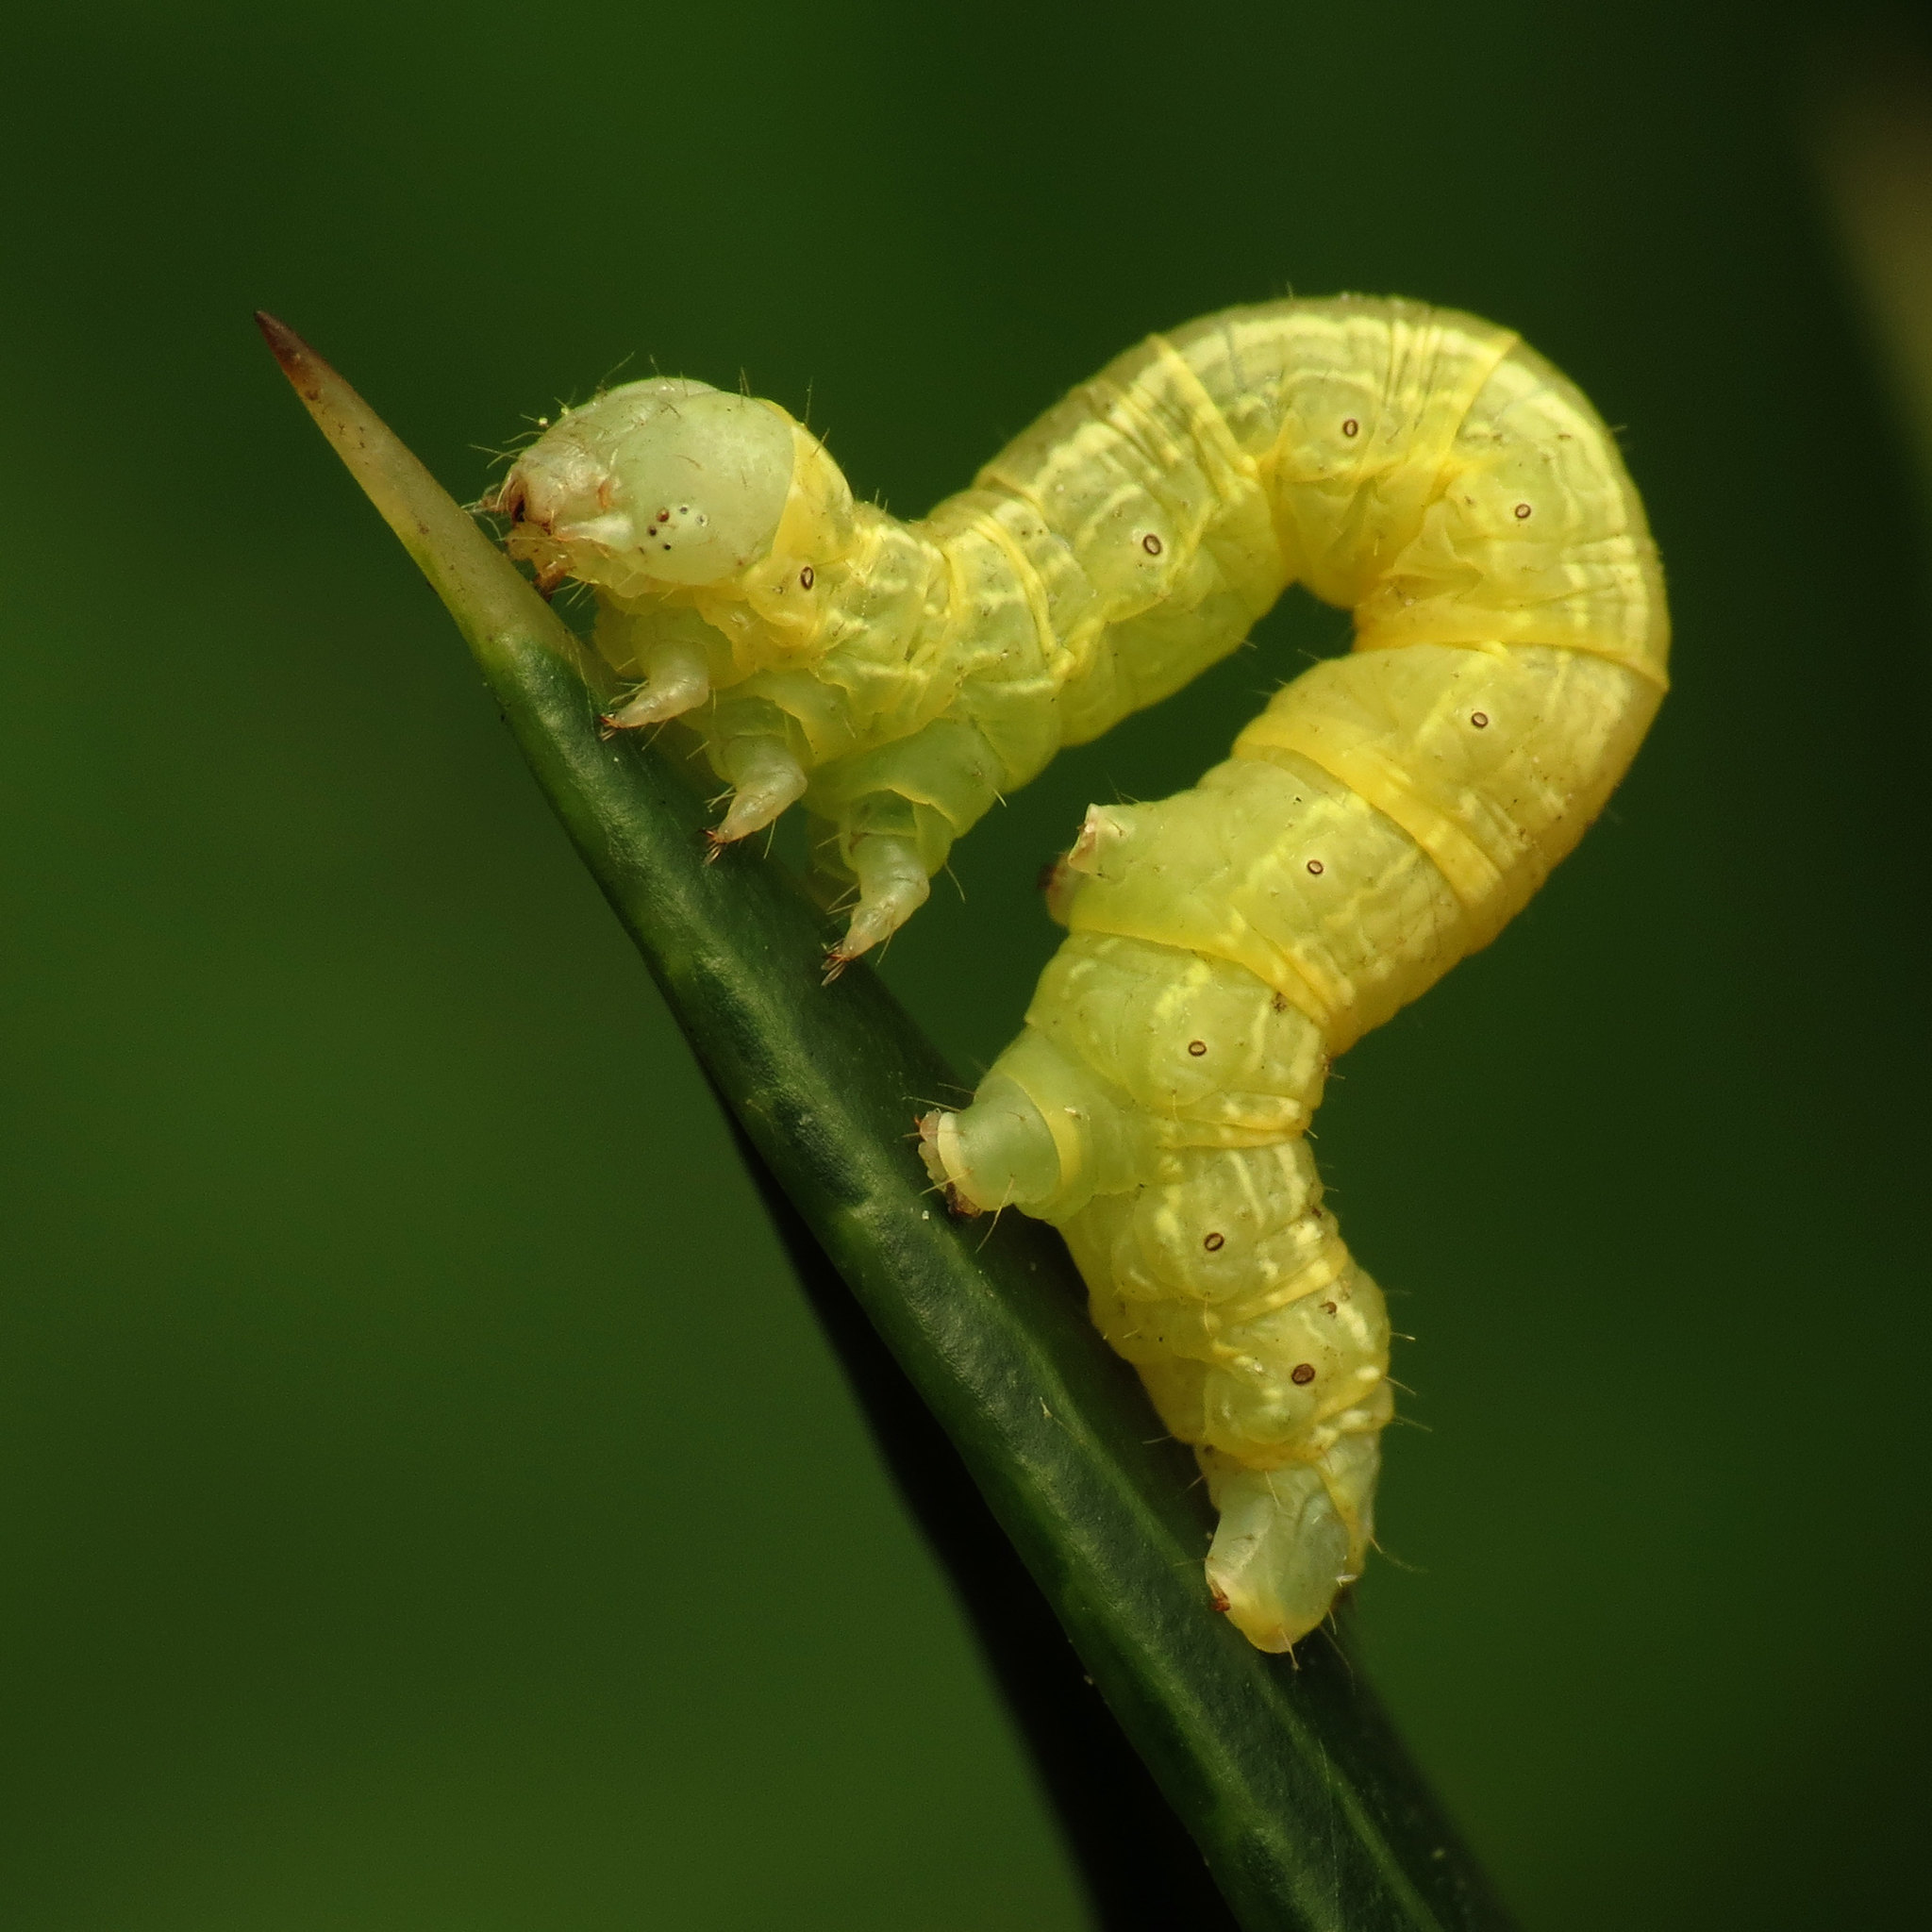
\includegraphics[width=160mm]{inchworm.jpg}
    \end{textblock*}
    \shadowedtitle{32mm}{7mm}{Incremental results}
\end{frame}


\begin{frame}
    \frametitle{Incremental results}
    \begin{center}
        In a typical commit, a small fraction of files in the repo change.
    \end{center}
    \begin{center}
        We want to reuse results that we've \\ already calculated for unchanged
        files.
    \end{center}
    \begin{center}
        \emph{Structural sharing} (like git itself) helps save storage.
    \end{center}
    \begin{center}
        \emph{Incremental processing} also helps save compute.
    \end{center}
\end{frame}


% incremental_separate_files
\begin{frame}[fragile]
    \frametitle{What would incremental results look like?}

    \uncover<1,2,4>{\highlightdef{def}}
    \uncover<1,3,4>{\highlightboth{import}}
    \uncover<1,3,4>{\highlightref{ref}}

    \begin{center}
    \begin{minipage}{21em}
    \begin{minipage}[t]{9em}
    \begin{uncoverenv}<1,2,4>
    \begin{minted}[label=stove.py]{python}
        def bake():
            pass

        def ?\tikzmark{def_start}?broil?\tikzmark{def_end}?():
            pass

        def saute():
            pass
    \end{minted}
    \end{uncoverenv}
    \end{minipage}
    \hspace{0.5em}
    \begin{minipage}[t]{11em}
    \begin{uncoverenv}<1,3,4>
    \begin{minted}[label=kitchen.py]{python}
        from stove import ?\tikzmark{import_start}?broil?\tikzmark{import_end}?

        ?\tikzmark{ref_start}?broil?\tikzmark{ref_end}?()
    \end{minted}
    \end{uncoverenv}
    \end{minipage}
    \end{minipage}
    \hspace{-7em}
    \begin{minipage}[t]{0.51\textwidth}
    \vskip 1em
    \begin{center}
        \uncover<3,4>{
            The reference at \textit{kitchen.py:3:1} \\
            refers to \texttt{stove.broil} in some other file
        }
        \\
        \uncover<4>{$+$}
        \\
        \uncover<2,4>{\texttt{stove.broil} is defined at \textit{stove.py:4:5}}
        \\
        \uncover<4>{$=$}
        \\
        \uncover<4>{
            The reference at \textit{kitchen.py:3:1} \\
            is defined at \textit{stove.py:4:5}
        }
    \end{center}
    \end{minipage}
    \end{center}
    \uncover<1,3,4>{\curvecodeline%
      [-]%
      {[yshift=10pt] pic cs:ref_end}%
      {+(45:1cm) and +(-155:1cm)}%
      {[yshift=-4pt] pic cs:import_start}%
    }
    \uncover<1,4>{\curvecodeline%
      {[xshift=12pt, yshift=10pt] pic cs:import_start}%
      {+(90:2cm) and +(75:2cm)}%
      {[xshift=-6pt, yshift=10pt] pic cs:def_end}%
    }
\end{frame}


\section{Stack graphs}

\begin{frame}
    \begin{textblock*}{160mm}(0mm,0mm)
        \picturecredit{Marco Verch}{Stack of pancakes with berries on a plate}{CC-BY-2.0}{https://flic.kr/p/2jYUh8M}
        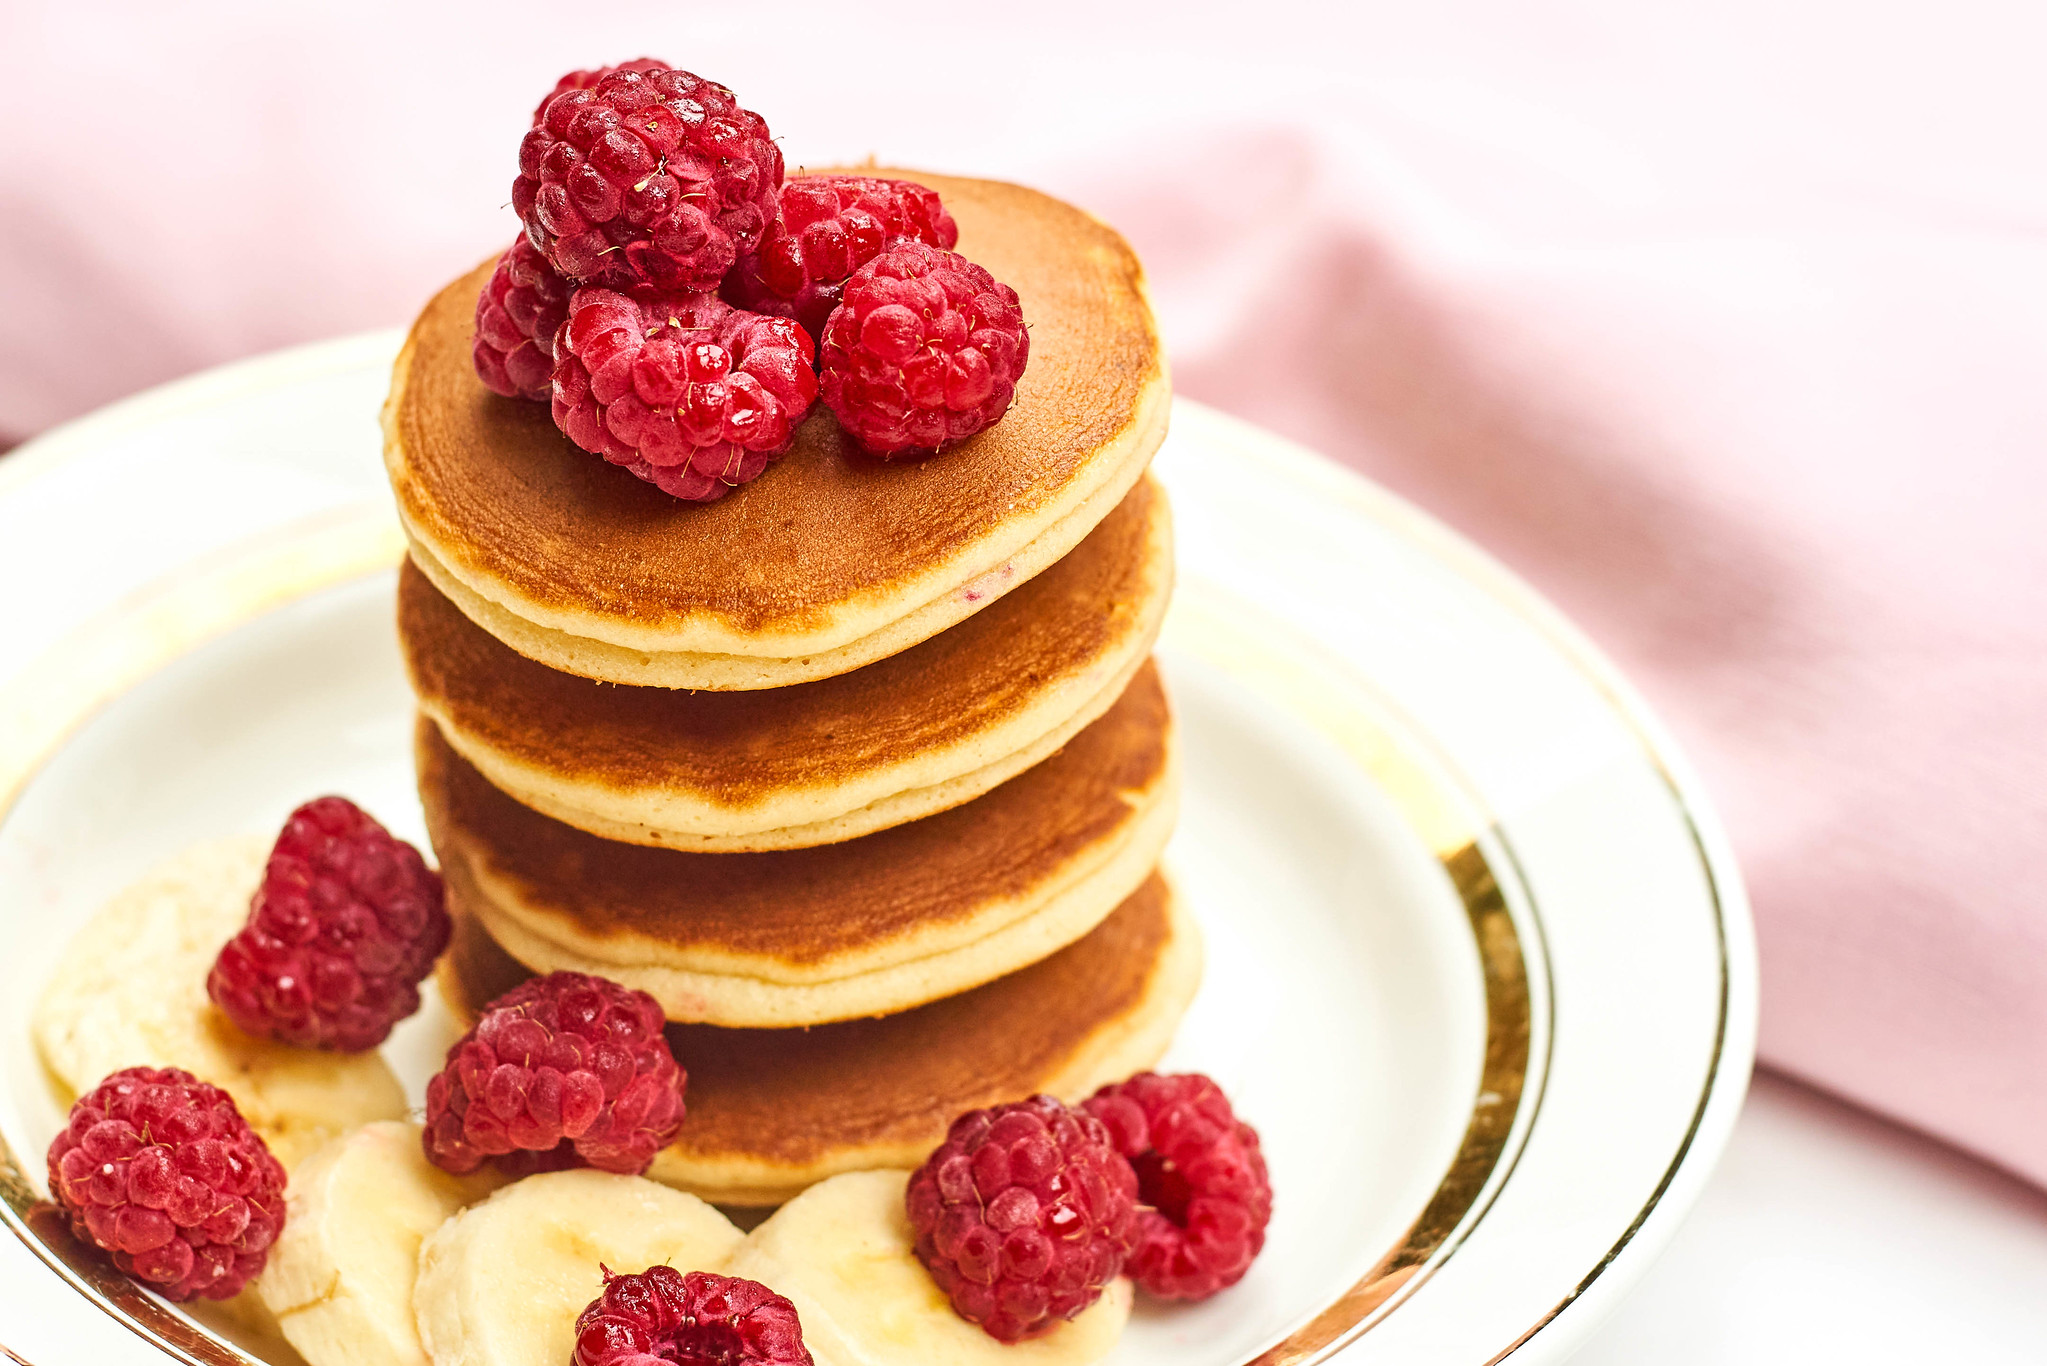
\includegraphics[width=160mm]{pancakes.jpg}
    \end{textblock*}
    \flattitle{110mm}{10mm}{Stack graphs}
\end{frame}


\begin{frame}[fragile]
    \frametitle{Stack graphs}
    \highlightdef{def}
    \highlightboth{import}
    \highlightref{ref}
    \begin{center}
    \begin{minipage}[t]{9em}
    \begin{minted}[label=stove.py]{python}
        def bake():
            pass

        def ?\tikzmark{def_start}?broil?\tikzmark{def_end}?():
            pass

        def saute():
            pass
    \end{minted}
    \end{minipage}
    \hspace{0.5em}
    \begin{minipage}[t]{11em}
    \begin{minted}[label=kitchen.py]{python}
        from stove import ?\tikzmark{import_start}?broil?\tikzmark{import_end}?

        ?\tikzmark{ref_start}?broil?\tikzmark{ref_end}?()
    \end{minted}
    \end{minipage}
    \end{center}
    \curvecodeline%
      [-]%
      {[yshift=10pt] pic cs:ref_end}%
      {+(45:1cm) and +(-155:1cm)}%
      {[yshift=-4pt] pic cs:import_start}%
    \curvecodeline%
      {[xshift=12pt, yshift=10pt] pic cs:import_start}%
      {+(90:2cm) and +(75:2cm)}%
      {[xshift=-6pt, yshift=10pt] pic cs:def_end}%
\end{frame}


\begin{frame}[fragile]
    \frametitle{Stack graphs}

    \uncover<3>{\highlightdef{def}}
    \uncover<5>{\highlightdef{mod}}

    \begin{center}

    \begin{minipage}{9em}
    \begin{minted}[label={\tikzmark{mod_start}stove.py\tikzmark{mod_end}}]{python}
        def bake():
            pass

        def ?\tikzmark{def_start}?broil?\tikzmark{def_end}?():
            pass

        def saute():
            pass
    \end{minted}
    \end{minipage}
    \hspace{2em}
    \begin{uncoverenv}<2- >
    \begin{tikzpicture}[baseline={(current bounding box.center)}]
        \node (root)       [highlight node on=<5>]
                           [root node]                            {};
        \node (stove)      [highlight node on=<5>]
                           [definition]  [left=of root]           {\PopSymbol{stove}};
        \node (dot)        [highlight node on=<5>]
                           [pop]         [left=of stove]          {\PopSymbol{.}};
        \node (s1)         [highlight node on=<4>]
                           [anon scope]  [left=of dot]            {};

        \setwidestsymbol{\PopSymbol{broil}}
        \node (s2)         [highlight node on=<4>]
                           [anon scope]  [above=\scopegap of s1]  {};
        \node (saute def)  [definition]  [left=of s2]             {\sized{\PopSymbol{saute}}};
        \node (s3)         [highlight node on=<4>]
                           [anon scope]  [above=\scopegap of s2]  {};
        \node (broil def)  [highlight node on=<3>]
                           [definition]  [left=of s3]             {\sized{\PopSymbol{broil}}};
        \node (s4)         [highlight node on=<4>]
                           [anon scope]  [above=\scopegap of s3]  {};
        \node (bake def)   [definition]  [left=of s4]             {\sized{\PopSymbol{bake}}};
        \node (s5)         [highlight node on=<4>]
                           [anon scope]  [above=\scopegap of s4]  {};

        \path [-Stealth]
          (root)      edge (stove)
          (stove)     edge (dot)
          (dot)       edge (s1)
          (s1)        edge (s2)
          (s2)        edge (s3)
                      edge (saute def)
          (s3)        edge (s4)
                      edge (broil def)
          (s4)        edge (s5)
                      edge (bake def)
          ;
    \end{tikzpicture}
    \end{uncoverenv}

    \end{center}
\end{frame}


\begin{frame}[fragile]
    \frametitle{Stack graphs}

    \uncover<3>{\highlightref{ref}}
    \uncover<4>{\highlightboth{import}}

    \begin{center}

    \begin{minipage}{11em}
    \begin{minted}[label=kitchen.py]{python}
        ?\tikzmark{import_start}?from stove import broil?\tikzmark{import_end}?

        ?\tikzmark{ref_start}?broil?\tikzmark{ref_end}?()
    \end{minted}
    \end{minipage}
    \hspace{-10em}
    \begin{uncoverenv}<2- >
    \begin{tikzpicture}[baseline={([yshift=2em] current bounding box.center)}]
        \node (root)       [highlight node on=<4>]
                           [root node]                            {};
        \node (kitchen)    [definition]  [right=of root]          {\PopSymbol{kitchen}};
        \node (dot)        [pop]         [right=of kitchen]       {\PopSymbol{.}};
        \node (k1)         [anon scope]  [right=of dot]           {};

        \node (k2)         [anon scope]  [above=\scopegap of k1]  {};
        \node (broil ref)  [highlight node on=<3>]
                           [reference]   [right=of k2]            {\PushSymbol{broil}};
        \node (k3)         [anon scope]  [above=\scopegap of k2]  {};
        \node (import def) [highlight node on=<4>]
                           [pop]         [right=of k3]            {\PopSymbol{broil}};
        \node (import ref) [highlight node on=<4>]
                           [push]        [right=of import def]    {\PushSymbol{broil}};
        \node (import dot) [highlight node on=<4>]
                           [push]        [right=of import ref]    {\PushSymbol{.}};
        \node (import mod) [highlight node on=<4>]
                           [push]        [right=of import dot]    {\PushSymbol{stove}};
        \node (k4)         [anon scope]  [above=\scopegap of k3]  {};

        \path [-Stealth]
          (root)      edge (kitchen)
          (kitchen)    edge (dot)
          (dot)        edge (k1)
          (k1)         edge (k2)
          (broil ref)  edge (k2)
          (k2)         edge (k3)
          (k3)         edge (k4)
                       edge (import def)
          (import def) edge (import ref)
          (import ref) edge (import dot)
          (import dot) edge (import mod)
          (import mod) edge [overlay, in control=+(-60:3cm), out control=+(-90:4cm)] (root)
          ;
    \end{tikzpicture}
    \end{uncoverenv}

    \end{center}
\end{frame}


% Combined

\begin{frame}[fragile]
    \frametitle{Stack graphs}
    \begin{center}
    \scalebox{0.75}{
    \begin{tikzpicture}
        \node (root)       [highlight node on={<2,3,13>}]
                           [root node]                            {};
        \node (stove)      [highlight node on={<2,14>}]
                           [definition]  [left=of root]           {\PopSymbol{stove}};
        \node (dot)        [highlight node on={<2,15>}]
                           [pop]         [left=of stove]          {\PopSymbol{.}};
        \node (s1)         [highlight node on={<2,16>}]
                           [anon scope]  [left=of dot]            {};

        \setwidestsymbol{\PopSymbol{broil}}
        \node (s2)         [highlight node on={<2,17>}]
                           [anon scope]  [above=\scopegap of s1]  {};
        \node (saute def)  [highlight node on=<2>]
                           [definition]  [left=of s2]             {\sized{\PopSymbol{saute}}};
        \node (s3)         [highlight node on={<2,18>}]
                           [anon scope]  [above=\scopegap of s2]  {};
        \node (broil def)  [highlight node on={<2,4,19>}]
                           [definition]  [left=of s3]             {\sized{\PopSymbol{broil}}};
        \node (s4)         [highlight node on=<2>]
                           [anon scope]  [above=\scopegap of s3]  {};
        \node (bake def)   [highlight node on=<2>]
                           [definition]  [left=of s4]             {\sized{\PopSymbol{bake}}};
        \node (s5)         [highlight node on=<2>]
                           [anon scope]  [above=\scopegap of s4]  {};

        \path [-Stealth]
          (root)      edge [highlight inner edge on=<4>, show path on=<14>] (stove)
          (stove)     edge [highlight inner edge on=<4>, show path on=<15>] (dot)
          (dot)       edge [highlight inner edge on=<4>, show path on=<16>] (s1)
          (s1)        edge [highlight inner edge on=<4>, show path on=<17>] (s2)
          (s2)        edge [highlight inner edge on=<4>, show path on=<18>] (s3)
                      edge (saute def)
          (s3)        edge (s4)
                      edge [highlight end edge on=<4>, show path on=<19>]   (broil def)
          (s4)        edge (s5)
                      edge (bake def)
          ;

        \node (kitchen)    [highlight node on=<3>]
                           [definition]  [right=of root]          {\PopSymbol{kitchen}};
        \node (dot)        [highlight node on=<3>]
                           [pop]         [right=of kitchen]       {\PopSymbol{.}};
        \node (k1)         [highlight node on=<3>]
                           [anon scope]  [right=of dot]           {};

        \node (k2)         [highlight node on={<3,7>}]
                           [anon scope]  [above=\scopegap of k1]  {};
        \node (broil ref)  [highlight node on={<3,4,6>}]
                           [reference]   [right=of k2]            {\PushSymbol{broil}};
        \node (k3)         [highlight node on={<3,8>}]
                           [anon scope]  [above=\scopegap of k2]  {};
        \node (import def) [highlight node on={<3,9>}]
                           [pop]         [right=of k3]            {\PopSymbol{broil}};
        \node (import ref) [highlight node on={<3,10>}]
                           [push]        [right=of import def]    {\PushSymbol{broil}};
        \node (import dot) [highlight node on={<3,11>}]
                           [push]        [right=of import ref]    {\PushSymbol{.}};
        \node (import mod) [highlight node on={<3,12>}]
                           [push]        [right=of import dot]    {\PushSymbol{stove}};
        \node (k4)         [highlight node on=<3>]
                           [anon scope]  [above=\scopegap of k3]  {};

        \path [-Stealth]
          (root)      edge (kitchen)
          (kitchen)    edge (dot)
          (dot)        edge (k1)
          (k1)         edge (k2)
          (broil ref)  edge [highlight inner edge on=<4>, show path on=<7>] (k2)
          (k2)         edge [highlight inner edge on=<4>, show path on=<8>] (k3)
          (k3)         edge (k4)
                       edge [highlight inner edge on=<4>, show path on=<9>] (import def)
          (import def) edge [highlight inner edge on=<4>, show path on=<10>] (import ref)
          (import ref) edge [highlight inner edge on=<4>, show path on=<11>] (import dot)
          (import dot) edge [highlight inner edge on=<4>, show path on=<12>] (import mod)
          (import mod) edge [overlay, in control=+(-60:3cm), out control=+(-90:4cm)]
                            [highlight inner edge on=<4>, show path on=<13>] (root)
          ;
    \end{tikzpicture}
    }
    \vskip 3em
    \begin{tabular}{m{5em} m{10em}}
        \only<5- >          {\textsmaller[2]{Symbol stack:}} &
        \only<6-8,10,15-18> {$\symbolstack{broil}$}
        \only<5,9,19>       {$\nilsymbolstack$}
        \only<11,14>        {$\symbolstack{.broil}$}
        \only<12-13>        {$\symbolstack{stove.broil}$}
        \\
    \end{tabular}
    \end{center}
\end{frame}


% Dataflow

\begin{frame}[fragile]
    \frametitle{The dataflow example}
    \begin{center}
    \begin{minipage}[t]{9em}
    \begin{minted}[label=dataflow.py]{python}
        def ?\tikzmark{passthrough_def_start}?passthrough(?\tikzmark{x_def_start}?x?\tikzmark{x_def_end}?):
            return ?\tikzmark{x_ref_start}?x?\tikzmark{x_ref_end}?
    \end{minted}
    \end{minipage}
    \hspace{0.5em}
    \begin{minipage}[t]{15em}
    \begin{minted}[label=a.py]{python}
        from dataflow import ?\tikzmark{passthrough_import_start}?passthrough?\tikzmark{passthrough_import_end}?

        class ?\tikzmark{A_def_start}?A?\tikzmark{A_def_end}?:
            ?\tikzmark{def_start}?one?\tikzmark{def_end}? = 1

        ?\tikzmark{passthrough_ref_start}?passthrough?\tikzmark{passthrough_ref_end}?(?\tikzmark{A_ref_start}?A?\tikzmark{A_ref_end}?).?\tikzmark{ref_start}?one?\tikzmark{ref_end}?
    \end{minted}
    \end{minipage}
    \end{center}
    \curvecodeline%
      [-]%
      {[yshift=-4pt] pic cs:ref_start}%
      {+(-135:0.5cm) and +(-75:0.5cm)}%
      {[xshift=15pt, yshift=-4pt] pic cs:passthrough_ref_start}%
    \curvecodeline%
      [-]%
      {[xshift=15pt, yshift=8pt] pic cs:passthrough_ref_start}%
      {+(75:1cm) and +(-90:1cm)}%
      {[xshift=15pt, yshift=-4pt] pic cs:passthrough_import_start}%
    \curvecodeline%
      [-]%
      {[xshift=15pt, yshift=8pt] pic cs:passthrough_import_start}%
      {+(90:1cm) and +(90:1cm)}%
      {[xshift=13pt, yshift=8pt] pic cs:passthrough_def_start}%
    \curvecodeline%
      [-]%
      {[xshift=15pt, yshift=-2pt] pic cs:passthrough_def_start}%
      {+(-45:0.25cm) and +(180:0.25cm)}%
      {[xshift=-2pt, yshift=3pt] pic cs:x_ref_start}%
    \curvecodeline%
      [-]%
      {[xshift=2pt, yshift=3pt] pic cs:x_ref_end}%
      {+(0:0.25cm) and +(180:0.25cm)}%
      {[xshift=-2pt, yshift=2pt] pic cs:x_def_start}%
    \curvecodeline%
      [-]%
      {[xshift=2pt, yshift=2pt] pic cs:x_def_end}%
      {+(0:4cm) and +(0:1cm)}%
      {[xshift=2pt, yshift=4pt] pic cs:A_ref_end}%
    \curvecodeline%
      [-]%
      {[xshift=-2pt, yshift=4pt] pic cs:A_ref_start}%
      {+(175:0.5cm) and +(-85:0.5cm)}%
      {[xshift=-1pt, yshift=-4pt] pic cs:A_def_end}%
    \curvecodeline%
      {[xshift=1pt, yshift=8pt] pic cs:A_def_start}%
      {+(105:0.5cm) and +(90:0.5cm)}%
      {[xshift=4pt, yshift=8pt] pic cs:def_start}%
\end{frame}

\begin{frame}[fragile]
    \frametitle{The dataflow example}
    \begin{center}
    \scalebox{0.6}{
    \begin{tikzpicture}
        \node (root)       [highlight node on={<2,3,17>}]
                           [root node]                            {};

        \node (a)          [highlight node on={<3>}]
                           [definition]  [right=2em of root]      {\PopSymbol{a}};
        \node (dot)        [highlight node on={<3>}]
                           [pop]         [above=of a]             {\PopSymbol{.}};
        \node (a1)         [highlight node on={<3>}]
                           [anon scope]  [above=\scopegap of dot] {};

        \node (a2)         [highlight node on={<3,10,33>}]
                           [anon scope]  [above=\scopegap of a1]  {};
        \node (pt ref)     [highlight node on={<3,9>}]
                           [reference]  [right=of a2]             {\PushSymbol{passthrough}};
        \node (call)       [highlight node on={<3,8>}]
                           [push]  [right=of pt ref]              {\PushScopedSymbol{()}{\scopestackelement{A}}};
        \node (member dot) [highlight node on={<3,7>}]
                           [push]  [right=of call]                {\PushSymbol{.}};
        \node (one ref)    [highlight node on={<3,4,6>}]
                           [reference]  [right=of member dot]     {\PushSymbol{one}};

        \node (A ref)      [highlight node on={<3,32>}]
                           [reference] [left=of a2]               {\PushSymbol{A}};
        \node (zero def)   [highlight node on={<3,31>}]
                           [pop]  [above=of A ref]                {\PopSymbol{0}};
        \node (actuals)    [highlight node on={<3,8,30>}]
                           [exported scope]  [above=of zero def]  {A};

        \node (a3)         [highlight node on={<3,11,34>}]
                           [anon scope]  [above=\scopegap of a2]  {};
        \node (A def)      [highlight node on={<3,35>}]
                           [definition]  [right=of a3]            {\PopSymbol{A}};
        \node (class)      [highlight node on={<3,36>}]
                           [exported scope]  [right=of A def]     {C};
        \node (class dot)  [highlight node on={<3,37>}]
                           [pop]  [right=of class]                {\PopSymbol{.}};
        \node (members)    [highlight node on={<3,38>}]
                           [anon scope]  [right=of class dot]     {};
        \node (one def)    [highlight node on={<3,4,39>}]
                           [definition]  [right=of members]       {\PopSymbol{one}};

        \node (a4)         [highlight node on={<3,12>}]
                           [anon scope]  [above=\scopegap of a3]  {};
        \node (import def) [highlight node on={<3,13>}]
                           [pop]  [right=of a4]                   {\PopSymbol{passthrough}};
        \node (import ref) [highlight node on={<3,14>}]
                           [push]  [right=of import def]          {\PushSymbol{passthrough}};
        \node (import dot) [highlight node on={<3,15>}]
                           [push]  [right=of import ref]          {\PushSymbol{.}};
        \node (import mod) [highlight node on={<3,16>}]
                           [push]  [right=of import dot]          {\PushSymbol{dataflow}};

        \node (a5)         [highlight node on={<3>}]
                           [anon scope]  [above=\scopegap of a4]  {};

        \path [-Stealth]
          (root)       edge (a)
          (a)          edge (dot)
          (dot)        edge (a1)
          (a1)         edge (a2)
          (one ref)    edge [highlight inner edge on=<4>, show path on=<7>]
                            (member dot)
          (member dot) edge [highlight inner edge on=<4>, show path on=<8>]
                            (call)
          (call)       edge [highlight inner edge on=<4>, show path on=<9>]
                            (pt ref)
          (pt ref)     edge [highlight inner edge on=<4>, show path on=<10>]
                            (a2)
          (a2)         edge [highlight inner edge on=<4>, show path on=<11>]
                            (a3)
          (a2)         edge [visible on={<4,34- >}]
                            [highlight inner edge on=<4>, show path on=<34>]
                            [out control=+(130:0.5cm), in control=+(-130:0.5cm)]
                            (a3)
          (actuals)    edge [highlight inner edge on=<4>, show path on=<31>]
                            (zero def)
          (zero def)   edge [highlight inner edge on=<4>, show path on=<32>]
                            (A ref)
          (A ref)      edge [highlight inner edge on=<4>, show path on=<33>]
                            (a2)
          (a3)         edge [highlight inner edge on=<4>, show path on=<35>]
                            (A def)
          (A def)      edge [highlight inner edge on=<4>, show path on=<36>]
                            (class)
          (class)      edge [highlight inner edge on=<4>, show path on=<37>]
                            (class dot)
          (class dot)  edge [highlight inner edge on=<4>, show path on=<38>]
                            (members)
          (members)    edge [highlight end edge on=<4>, show path on=<39>]
                            (one def)
          (a3)         edge [highlight inner edge on=<4>, show path on=<12>]
                            (a4)
          (a4)         edge [highlight inner edge on=<4>, show path on=<13>]
                            (import def)
          (import def) edge [highlight inner edge on=<4>, show path on=<14>]
                            (import ref)
          (import ref) edge [highlight inner edge on=<4>, show path on=<15>]
                            (import dot)
          (import dot) edge [highlight inner edge on=<4>, show path on=<16>]
                            (import mod)
          (import mod) edge [overlay, in control=+(-45:2cm), out control=+(-90:9cm)]
                            [highlight inner edge on=<4>, show path on=<17>]
                            (root)
          (a4)         edge (a5)
          ;

        \node (dataflow)   [highlight node on={<2,18>}]
                           [definition]  [left=2em of root]       {\PopSymbol{dataflow}};
        \node (dot)        [highlight node on={<2,19>}]
                           [pop]         [above=of dataflow]      {\PopSymbol{.}};
        \node (d1)         [highlight node on={<2,20>}]
                           [anon scope]  [left=\scopegap of dot] {};

        \node (d2)         [highlight node on={<2,21>}]
                           [anon scope]  [above=\scopegap of d1]  {};
        \node (pt def)     [highlight node on={<2,22>}]
                           [definition]  [left=of d2]             {\PopSymbol{passthrough}};
        \node (called)     [highlight node on={<2,23>}]
                           [pop]  [left=of pt def]                {\PopScopedSymbol{()}};
        \node (ret)        [highlight node on={<2,24>}]
                           [exported scope]  [above=of called]    {R};
        \node (x ref)      [highlight node on={<2,25>}]
                           [reference]  [above=of ret]            {\PushSymbol{x}};
        \node (formals)    [highlight node on={<2,26>}]
                           [exported scope]  [above=of x ref]     {F};
        \node (x def)      [highlight node on={<2,27>}]
                           [pop]  [right=of formals]              {\PopSymbol{x}};
        \node (x param)    [highlight node on={<2>}]
                           [push]  [right=of x def]               {\PushSymbol{x}};
        \node (zero param) [highlight node on={<2,28>}]
                           [push]  [above=of x param]             {\PushSymbol{0}};
        \node (x jump)     [highlight node on={<2,29>}]
                           [control node] [right=of zero param]   {JUMP};

        \node (d3)         [highlight node on={<2>}]
                           [anon scope]  [above=\scopegap of d2]  {};

        \path [-Stealth]
          (root)       edge [highlight inner edge on=<4>, show path on=<18>]
                            (dataflow)
          (dataflow)   edge [highlight inner edge on=<4>, show path on=<19>]
                            (dot)
          (dot)        edge [highlight inner edge on=<4>, show path on=<20>]
                            (d1)
          (d1)         edge [highlight inner edge on=<4>, show path on=<21>]
                            (d2)
          (d2)         edge [highlight inner edge on=<4>, show path on=<22>]
                            (pt def)
          (pt def)     edge [highlight inner edge on=<4>, show path on=<23>]
                            (called)
          (called)     edge [highlight inner edge on=<4>, show path on=<24>]
                            (ret)
          (ret)        edge [highlight inner edge on=<4>, show path on=<25>]
                            (x ref)
          (x ref)      edge [highlight inner edge on=<4>, show path on=<26>]
                            (formals)
          (formals)    edge [highlight inner edge on=<4>, show path on=<27>]
                            (x def)
          (x def)      edge (x param)
          (x def)      edge [highlight inner edge on=<4>, show path on=<28>]
                            (zero param)
          (x param)    edge (x jump)
          (zero param) edge [highlight inner edge on=<4>, show path on=<29>]
                            (x jump)
          (x jump)     edge [in control=+(135:1cm), out control=+(0:1cm)]
                            [visible on={<4,30- >}]
                            [highlight inner edge on=<4>, show path on=<30>]
                            [dotted]
                            (actuals)
          (d2)         edge (d3)
          ;

    \end{tikzpicture}
    }
    \vskip 2em
    \begin{tabular}{m{5em} m{14em}}
        \only<5- >                 {\textsmaller[2]{Symbol stack:}} &
        \only<5,39>                {$\nilsymbolstack$}
        \only<6,37-38>             {$\symbolstack{one}$}
        \only<7,23-24,27,31,35-36> {$\symbolstack{.one}$}
        \only<8,13,22>             {$\symbolstack{$\scoped{()}{\scopestackelement{A}}$.one}$}
        \only<9-12,14,19-21>       {$\symbolstack{passthrough$\scoped{()}{\scopestackelement{A}}$.one}$}
        \only<15,18>               {$\symbolstack{.passthrough$\scoped{()}{\scopestackelement{A}}$.one}$}
        \only<16-17>               {$\symbolstack{dataflow.passthrough$\scoped{()}{\scopestackelement{A}}$.one}$}
        \only<25-26>               {$\symbolstack{x.one}$}
        \only<28-30>               {$\symbolstack{0.one}$}
        \only<32-34>               {$\symbolstack{A.one}$}
        \\
        \only<5- >                 {\textsmaller[2]{Scope stack:}} &
        \only<5-22,30- >           {$\nilscopestack$}
        \only<23-29>               {$\scopestack{\scopestackelement{A}}$}
        \\
    \end{tabular}
    \end{center}
\end{frame}


\begin{frame}[t]
    \frametitle{Are we done?}
    \vskip 2em
    \begin{tikzpicture}
        \node (bar) at(0,0) [
            rectangle, anchor=west,
            minimum width=\columnwidth, minimum height=1cm,
            draw=black, thin,
            fill=gray!20,
        ] {};

        \node (query) at(bar.east) [
            rectangle, anchor=east,
            minimum width=0.8\columnwidth, minimum height=1cm,
            draw=black, thin,
            fill=blue!20,
        ] {};

        \node at(bar.west) [
            rectangle, anchor=west, inner xsep=2ex,
            text height=1.5ex, text depth=0.25ex,
            text=black,
        ] {Index};
        \node at(bar.east) [
            rectangle, anchor=east, inner xsep=2ex,
            text height=1.5ex, text depth=0.25ex,
            text=black,
        ] {Query};
    \end{tikzpicture}

    \begin{center}
        We're still doing too much work at query time!
    \end{center}

    \begin{center}
        Can we shift more of the work to index time, \\
        while still remaining incremental?
    \end{center}
\end{frame}


\section{Partial paths}

\begin{frame}
    \begin{textblock*}{160mm}(0mm,0mm)
        \picturecredit{Seattle Municipal Archives}{West Seattle Bridge under construction, circa 1983}{CC-BY-2.0}{https://flic.kr/p/7jKWYi}
        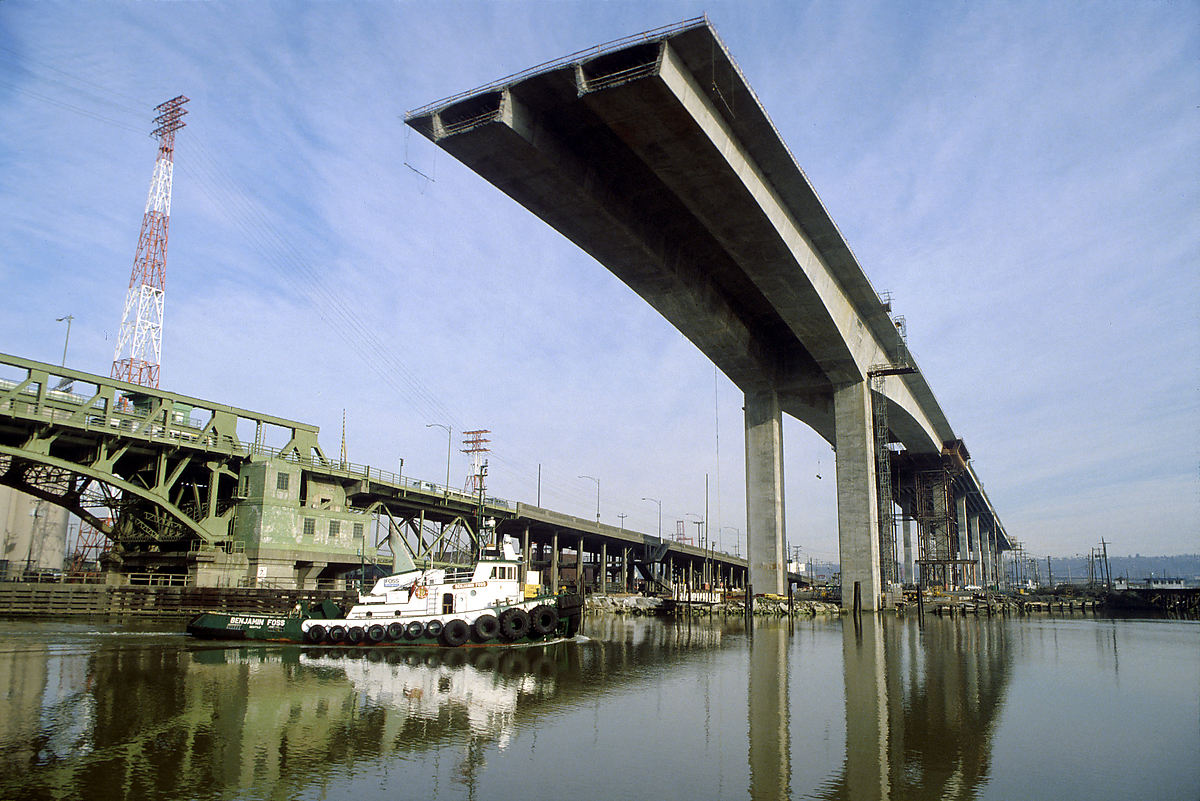
\includegraphics[width=160mm]{bridge.jpg}
    \end{textblock*}
    \shadowedtitle{150mm - \titlewidth}{10mm}{Partial paths}
\end{frame}


\begin{frame}[fragile]
    \frametitle{Partial paths}

    \begin{center}

    \begin{minipage}{11em}
    \begin{minted}[label=kitchen.py]{python}
        ?\tikzmark{import_start}?from stove import broil?\tikzmark{import_end}?

        ?\tikzmark{ref_start}?broil?\tikzmark{ref_end}?()
    \end{minted}
    \end{minipage}
    \hspace{-2em}
    \scalebox{0.75}{
    \begin{tikzpicture}[baseline={([yshift=1em] current bounding box.center)}]
        \node (root)       [root node]                            {};
        \node (kitchen)    [definition]  [right=of root]          {\PopSymbol{kitchen}};
        \node (dot)        [pop]         [right=of kitchen]       {\PopSymbol{.}};
        \node (k1)         [anon scope]  [right=of dot]           {};

        \node (k2)         [anon scope]  [above=\scopegap of k1]  {};
        \node (broil ref)  [reference]   [right=of k2]            {\PushSymbol{broil}};
        \node (k3)         [anon scope]  [above=\scopegap of k2]  {};
        \node (import def) [pop]         [right=of k3]            {\PopSymbol{broil}};
        \node (import ref) [push]        [right=of import def]    {\PushSymbol{broil}};
        \node (import dot) [push]        [right=of import ref]    {\PushSymbol{.}};
        \node (import mod) [push]        [right=of import dot]    {\PushSymbol{stove}};
        \node (k4)         [anon scope]  [above=\scopegap of k3]  {};

        \path [-Stealth]
          (root)      edge (kitchen)
          (kitchen)    edge (dot)
          (dot)        edge (k1)
          (k1)         edge (k2)
          (broil ref)  edge [highlight inner edge on=<2- >] (k2)
          (k2)         edge [highlight inner edge on=<2- >] (k3)
          (k3)         edge (k4)
                       edge [highlight inner edge on=<2- >] (import def)
          (import def) edge [highlight inner edge on=<2- >] (import ref)
          (import ref) edge [highlight inner edge on=<2- >] (import dot)
          (import dot) edge [highlight inner edge on=<2- >] (import mod)
          (import mod) edge [highlight end edge on=<2- >]
                            [overlay, in control=+(-60:3cm), out control=+(-90:4cm)] (root)
          ;
    \end{tikzpicture}
    }

    \vskip 5em
    \uncover<3- >{\partialpath
        {\nilsymbolstack}{\nilscopestack}
        {\node [reference] {\PushSymbol{broil}}}
        {\node [root node] {}}
        {\symbolstack{stove.broil}}{\nilscopestack}}
    \vskip 0.75em
    \uncover<4>{The reference at \textit{kitchen.py:3:1}  refers to \texttt{stove.broil} in some other file}

    \end{center}
\end{frame}


\begin{frame}[fragile]
    \frametitle{Partial paths}

    \begin{center}

    \begin{minipage}{9em}
    \begin{minted}[label={\tikzmark{mod_start}stove.py\tikzmark{mod_end}}]{python}
        def bake():
            pass

        def ?\tikzmark{def_start}?broil?\tikzmark{def_end}?():
            pass

        def saute():
            pass
    \end{minted}
    \end{minipage}
    \hspace{2em}
    \scalebox{0.75}{
    \begin{tikzpicture}[baseline={(current bounding box.center)}]
        \node (root)       [root node]                            {};
        \node (stove)      [definition]  [left=of root]           {\PopSymbol{stove}};
        \node (dot)        [pop]         [left=of stove]          {\PopSymbol{.}};
        \node (s1)         [anon scope]  [left=of dot]            {};

        \setwidestsymbol{\PopSymbol{broil}}
        \node (s2)         [anon scope]  [above=\scopegap of s1]  {};
        \node (saute def)  [definition]  [left=of s2]             {\sized{\PopSymbol{saute}}};
        \node (s3)         [anon scope]  [above=\scopegap of s2]  {};
        \node (broil def)  [definition]  [left=of s3]             {\sized{\PopSymbol{broil}}};
        \node (s4)         [anon scope]  [above=\scopegap of s3]  {};
        \node (bake def)   [definition]  [left=of s4]             {\sized{\PopSymbol{bake}}};
        \node (s5)         [anon scope]  [above=\scopegap of s4]  {};

        \path [-Stealth]
          (root)      edge [highlight inner edge on=<2- >] (stove)
          (stove)     edge [highlight inner edge on=<2- >] (dot)
          (dot)       edge [highlight inner edge on=<2- >] (s1)
          (s1)        edge [highlight inner edge on=<2- >] (s2)
          (s2)        edge [highlight inner edge on=<2- >] (s3)
                      edge (saute def)
          (s3)        edge (s4)
                      edge [highlight end edge on=<2- >] (broil def)
          (s4)        edge (s5)
                      edge (bake def)
          ;
    \end{tikzpicture}
    }

    \vskip 2em
    \uncover<3- >{\partialpath
        {\symbolstack{stove.broil} \cdot \psi}{\phi}
        {\node [root node] {}}
        {\node [definition] {\PopSymbol{broil}}}
        {\psi}{\phi}}
    \vskip 0.75em
    \uncover<4>{\texttt{stove.broil} is defined at \textit{stove.py:4:5}.}

    \end{center}
\end{frame}


\begin{frame}[fragile]
    \frametitle{Concatenating partial paths}

    \vskip 2em
    \begin{center}
        \begin{minipage}[t]{0.46\textwidth}
            \begin{center}
            \scalebox{0.75}{\partialpath
                {\nilsymbolstack}{\nilscopestack}
                {\node [reference] {\PushSymbol{broil}}}
                {\node [root node] {}}
                {\symbolstack{stove.broil}}{\nilscopestack}}
            \end{center}
        \end{minipage}
            \; $+$ \;
        \begin{minipage}[t]{0.46\textwidth}
            \begin{center}
            \scalebox{0.75}{\partialpath
                {\symbolstack{stove.broil} \cdot \psi}{\phi}
                {\node [root node] {}}
                {\node [definition] {\PopSymbol{broil}}}
                {\psi}{\phi}}
            \end{center}
        \end{minipage}
        \vskip 0.5em
        \begin{minipage}[t][1cm][t]{0.46\textwidth}
        \begin{center}
            \scalebox{0.75}{
                \onslide<2>{$\psi = \nilsymbolstack, \phi = \nilscopestack$}
            }
        \end{center}
        \end{minipage}
        \vskip 0.5em
        \begin{minipage}[c][2cm][c]{0.46\textwidth}
            \begin{center}
            \smaller[1]
            The reference at \textit{kitchen.py:3:1} \\
            refers to \texttt{stove.broil} in some other file
            \end{center}
        \end{minipage}
            \; $+$ \;
        \begin{minipage}[c][2cm][c]{0.46\textwidth}
            \begin{center}
            \smaller[1]
            \texttt{stove.broil} is defined at \textit{stove.py:4:5}
            \end{center}
        \end{minipage}
    \end{center}
\end{frame}


\begin{frame}[fragile]
    \frametitle{Concatenating partial paths}

    \vskip 2em
    \begin{center}
        \begin{minipage}[t]{\textwidth}
            \begin{center}
            \scalebox{0.75}{\partialpath
                {\nilsymbolstack}{\nilscopestack}
                {\node [reference] {\PushSymbol{broil}}}
                {\node [definition] {\PopSymbol{broil}}}
                {\nilsymbolstack}{\nilscopestack}}
            \end{center}
        \end{minipage}
        \vskip 0.5em
        \begin{minipage}[t][1cm][t]{0.46\textwidth}
            \scalebox{0.75}{
                \vphantom{$\psi = \nilsymbolstack, \phi = \nilscopestack$}
            }
        \end{minipage}
        \vskip 0.5em
        \begin{minipage}[c][2cm][c]{0.46\textwidth}
            \begin{center}
            \smaller[1]
            The reference at \textit{kitchen.py:3:1} \\
            is defined at \textit{stove.py:4:5}. \\
            \end{center}
        \end{minipage}
    \end{center}
\end{frame}


\begin{frame}[t,fragile]
    \frametitle{The dataflow example}

    \begin{center}

    \begin{minipage}{9em}
    \begin{minted}[label=dataflow.py]{python}
        def ?\tikzmark{passthrough_def_start}?passthrough(?\tikzmark{x_def_start}?x?\tikzmark{x_def_end}?):
            return ?\tikzmark{x_ref_start}?x?\tikzmark{x_ref_end}?
    \end{minted}
    \end{minipage}
    \hspace{2em}
    \scalebox{0.6}{
    \begin{tikzpicture}[baseline={([yshift=1em] current bounding box.center)}]
        \node (root)       [root node]                            {};

        \node (dataflow)   [definition]  [left=2em of root]       {\PopSymbol{dataflow}};
        \node (dot)        [pop]         [above=of dataflow]      {\PopSymbol{.}};
        \node (d1)         [anon scope]  [left=\scopegap of dot] {};

        \node (d2)         [anon scope]  [above=\scopegap of d1]  {};
        \node (pt def)     [definition]  [left=of d2]             {\PopSymbol{passthrough}};
        \node (called)     [pop]  [left=of pt def]                {\PopScopedSymbol{()}};
        \node (ret)        [exported scope]  [above=of called]    {R};
        \node (x ref)      [reference]  [above=of ret]            {\PushSymbol{x}};
        \node (formals)    [exported scope]  [above=of x ref]     {F};
        \node (x def)      [pop]  [right=of formals]              {\PopSymbol{x}};
        \node (x param)    [push]  [right=of x def]               {\PushSymbol{x}};
        \node (zero param) [push]  [above=of x param]             {\PushSymbol{0}};
        \node (x jump)     [control node] [right=of zero param]   {JUMP};

        \node (d3)         [anon scope]  [above=\scopegap of d2]  {};

        \path [-Stealth]
          (root)       edge [highlight inner edge on=<2- >]
                            (dataflow)
          (dataflow)   edge [highlight inner edge on=<2- >]
                            (dot)
          (dot)        edge [highlight inner edge on=<2- >]
                            (d1)
          (d1)         edge [highlight inner edge on=<2- >]
                            (d2)
          (d2)         edge [highlight inner edge on=<2- >]
                            (pt def)
          (pt def)     edge [highlight inner edge on=<2- >]
                            (called)
          (called)     edge [highlight end edge on=<2- >]
                            (ret)
          (ret)        edge (x ref)
          (x ref)      edge (formals)
          (formals)    edge (x def)
          (x def)      edge (x param)
          (x def)      edge (zero param)
          (x param)    edge (x jump)
          (zero param) edge (x jump)
          (d2)         edge (d3)
          ;
    \end{tikzpicture}
    }
    \hspace{3em}

    \vskip 1em
    \uncover<3- >{\partialpath
        {\symbolstack{dataflow.passthrough$\scoped{\texttt{()}}{\phi_A}$} \cdot \psi}{\phi}
        {\node [root node]{}}
        {\node [exported scope] {R}}
        {\psi}{\phi_A}}
    \vskip 0.75em
    \uncover<4>{
        \texttt{dataflow.passthrough} is a function \\
        that can be invoked. \\
    }

    \end{center}
\end{frame}


\begin{frame}[t,fragile]
    \frametitle{The dataflow example}

    \begin{center}

    \begin{minipage}{9em}
    \begin{minted}[label=dataflow.py]{python}
        def ?\tikzmark{passthrough_def_start}?passthrough(?\tikzmark{x_def_start}?x?\tikzmark{x_def_end}?):
            return ?\tikzmark{x_ref_start}?x?\tikzmark{x_ref_end}?
    \end{minted}
    \end{minipage}
    \hspace{2em}
    \scalebox{0.6}{
    \begin{tikzpicture}[baseline={([yshift=1em] current bounding box.center)}]
        \node (root)       [root node]                            {};

        \node (dataflow)   [definition]  [left=2em of root]       {\PopSymbol{dataflow}};
        \node (dot)        [pop]         [above=of dataflow]      {\PopSymbol{.}};
        \node (d1)         [anon scope]  [left=\scopegap of dot] {};

        \node (d2)         [anon scope]  [above=\scopegap of d1]  {};
        \node (pt def)     [definition]  [left=of d2]             {\PopSymbol{passthrough}};
        \node (called)     [pop]  [left=of pt def]                {\PopScopedSymbol{()}};
        \node (ret)        [exported scope]  [above=of called]    {R};
        \node (x ref)      [reference]  [above=of ret]            {\PushSymbol{x}};
        \node (formals)    [exported scope]  [above=of x ref]     {F};
        \node (x def)      [pop]  [right=of formals]              {\PopSymbol{x}};
        \node (x param)    [push]  [right=of x def]               {\PushSymbol{x}};
        \node (zero param) [push]  [above=of x param]             {\PushSymbol{0}};
        \node (x jump)     [control node] [right=of zero param]   {JUMP};

        \node (d3)         [anon scope]  [above=\scopegap of d2]  {};

        \path [-Stealth]
          (root)       edge (dataflow)
          (dataflow)   edge (dot)
          (dot)        edge (d1)
          (d1)         edge (d2)
          (d2)         edge (pt def)
          (pt def)     edge (called)
          (called)     edge (ret)
          (ret)        edge [highlight inner edge on=<2- >]
                            (x ref)
          (x ref)      edge [highlight inner edge on=<2- >]
                            (formals)
          (formals)    edge [highlight inner edge on=<2- >]
                            (x def)
          (x def)      edge (x param)
          (x def)      edge [highlight inner edge on=<2- >]
                            (zero param)
          (x param)    edge (x jump)
          (zero param) edge [highlight end edge on=<2- >]
                            (x jump)
          (d2)         edge (d3)
          ;
    \end{tikzpicture}
    }
    \hspace{3em}

    \vskip 1em
    \uncover<3- >{\partialpath
        {\psi}{\phi}
        {\node [exported scope] {R}}
        {\node [control node]{JUMP}}
        {\symbolstack{0} \cdot \psi}{\phi}}
    \vskip 0.75em
    \uncover<4>{
        The return value of \texttt{dataflow.passthrough} \\
        has the same type as positional parameter 0. \\
    }

    \end{center}
\end{frame}


\begin{frame}[t,fragile]
    \frametitle{The dataflow example}

    \begin{center}

    \begin{minipage}[t]{15em}
    \begin{minted}[label=a.py]{python}
        from dataflow import ?\tikzmark{passthrough_import_start}?passthrough?\tikzmark{passthrough_import_end}?

        class ?\tikzmark{A_def_start}?A?\tikzmark{A_def_end}?:
            ?\tikzmark{def_start}?one?\tikzmark{def_end}? = 1

        ?\tikzmark{passthrough_ref_start}?passthrough?\tikzmark{passthrough_ref_end}?(?\tikzmark{A_ref_start}?A?\tikzmark{A_ref_end}?).?\tikzmark{ref_start}?one?\tikzmark{ref_end}?
    \end{minted}
    \end{minipage}
    \hspace{2em}
    \scalebox{0.6}{
    \begin{tikzpicture}[baseline={([yshift=4em] current bounding box.center)}]
        \node (root)       [root node]                            {};

        \node (a)          [definition]  [left=2em of root]       {\PopSymbol{a}};
        \node (dot)        [pop]         [left=of a]              {\PopSymbol{.}};
        \node (a1)         [anon scope]  [left=\scopegap of dot]  {};

        \node (a2)         [anon scope]  [above=\scopegap of a1]  {};
        \node (pt ref)     [reference]  [right=of a2]             {\PushSymbol{passthrough}};
        \node (call)       [push]  [right=of pt ref]              {\PushScopedSymbol{()}{\scopestackelement{A}}};
        \node (member dot) [push]  [right=of call]                {\PushSymbol{.}};
        \node (one ref)    [reference]  [right=of member dot]     {\PushSymbol{one}};

        \node (A ref)      [reference] [left=of a2]               {\PushSymbol{A}};
        \node (zero def)   [pop]  [above=of A ref]                {\PopSymbol{0}};
        \node (actuals)    [exported scope]  [above=of zero def]  {A};

        \node (a3)         [anon scope]  [above=\scopegap of a2]  {};
        \node (A def)      [definition]  [right=of a3]            {\PopSymbol{A}};
        \node (class)      [exported scope]  [right=of A def]     {C};
        \node (class dot)  [pop]  [right=of class]                {\PopSymbol{.}};
        \node (members)    [anon scope]  [right=of class dot]     {};
        \node (one def)    [definition]  [right=of members]       {\PopSymbol{one}};

        \node (a4)         [anon scope]  [above=\scopegap of a3]  {};
        \node (import def) [pop]  [right=of a4]                   {\PopSymbol{passthrough}};
        \node (import ref) [push]  [right=of import def]          {\PushSymbol{passthrough}};
        \node (import dot) [push]  [right=of import ref]          {\PushSymbol{.}};
        \node (import mod) [push]  [right=of import dot]          {\PushSymbol{dataflow}};

        \node (a5)         [anon scope]  [above=\scopegap of a4]  {};

        \path [-Stealth]
          (root)       edge (a)
          (a)          edge (dot)
          (dot)        edge (a1)
          (a1)         edge (a2)
          (one ref)    edge [highlight inner edge on=<2- >]
                            (member dot)
          (member dot) edge [highlight inner edge on=<2- >]
                            (call)
          (call)       edge [highlight inner edge on=<2- >]
                            (pt ref)
          (pt ref)     edge [highlight inner edge on=<2- >]
                            (a2)
          (a2)         edge [highlight inner edge on=<2- >]
                            (a3)
          (actuals)    edge (zero def)
          (zero def)   edge (A ref)
          (A ref)      edge (a2)
          (a3)         edge (A def)
          (A def)      edge (class)
          (class)      edge (class dot)
          (class dot)  edge (members)
          (members)    edge (one def)
          (a3)         edge [highlight inner edge on=<2- >]
                            (a4)
          (a4)         edge [highlight inner edge on=<2- >]
                            (import def)
          (import def) edge [highlight inner edge on=<2- >]
                            (import ref)
          (import ref) edge [highlight inner edge on=<2- >]
                            (import dot)
          (import dot) edge [highlight inner edge on=<2- >]
                            (import mod)
          (import mod) edge [overlay, in control=+(5:4cm), out control=+(-90:4cm)]
                            [highlight end edge on=<2- >]
                            (root)
          (a4)         edge (a5)
          ;
    \end{tikzpicture}
    }
    \hspace{3em}

    \vskip 2em
    \uncover<3- >{\partialpath
        {\nilsymbolstack}{\nilscopestack}
        {\node [reference] {one}}
        {\node [root node]{}}
        {\symbolstack{dataflow.passthrough$\scoped{()}{\scopestackelement{A}}$.one}}{\nilscopestack}}
    \vskip 0.75em
    \uncover<4>{
        If you can find what \texttt{dataflow.passthrough} resolves to and can call it \\
        then the result should have a member named \texttt{one} \\
        which the reference at \textit{a.py:6:16} resolves to. \\
    }

    \end{center}
\end{frame}


\begin{frame}[t,fragile]
    \frametitle{The dataflow example}

    \begin{center}

    \begin{minipage}[t]{15em}
    \begin{minted}[label=a.py]{python}
        from dataflow import ?\tikzmark{passthrough_import_start}?passthrough?\tikzmark{passthrough_import_end}?

        class ?\tikzmark{A_def_start}?A?\tikzmark{A_def_end}?:
            ?\tikzmark{def_start}?one?\tikzmark{def_end}? = 1

        ?\tikzmark{passthrough_ref_start}?passthrough?\tikzmark{passthrough_ref_end}?(?\tikzmark{A_ref_start}?A?\tikzmark{A_ref_end}?).?\tikzmark{ref_start}?one?\tikzmark{ref_end}?
    \end{minted}
    \end{minipage}
    \hspace{2em}
    \scalebox{0.6}{
    \begin{tikzpicture}[baseline={([yshift=4em] current bounding box.center)}]
        \node (root)       [root node]                            {};

        \node (a)          [definition]  [left=2em of root]       {\PopSymbol{a}};
        \node (dot)        [pop]         [left=of a]              {\PopSymbol{.}};
        \node (a1)         [anon scope]  [left=\scopegap of dot]  {};

        \node (a2)         [anon scope]  [above=\scopegap of a1]  {};
        \node (pt ref)     [reference]  [right=of a2]             {\PushSymbol{passthrough}};
        \node (call)       [push]  [right=of pt ref]              {\PushScopedSymbol{()}{\scopestackelement{A}}};
        \node (member dot) [push]  [right=of call]                {\PushSymbol{.}};
        \node (one ref)    [reference]  [right=of member dot]     {\PushSymbol{one}};

        \node (A ref)      [reference] [left=of a2]               {\PushSymbol{A}};
        \node (zero def)   [pop]  [above=of A ref]                {\PopSymbol{0}};
        \node (actuals)    [exported scope]  [above=of zero def]  {A};

        \node (a3)         [anon scope]  [above=\scopegap of a2]  {};
        \node (A def)      [definition]  [right=of a3]            {\PopSymbol{A}};
        \node (class)      [exported scope]  [right=of A def]     {C};
        \node (class dot)  [pop]  [right=of class]                {\PopSymbol{.}};
        \node (members)    [anon scope]  [right=of class dot]     {};
        \node (one def)    [definition]  [right=of members]       {\PopSymbol{one}};

        \node (a4)         [anon scope]  [above=\scopegap of a3]  {};
        \node (import def) [pop]  [right=of a4]                   {\PopSymbol{passthrough}};
        \node (import ref) [push]  [right=of import def]          {\PushSymbol{passthrough}};
        \node (import dot) [push]  [right=of import ref]          {\PushSymbol{.}};
        \node (import mod) [push]  [right=of import dot]          {\PushSymbol{dataflow}};

        \node (a5)         [anon scope]  [above=\scopegap of a4]  {};

        \path [-Stealth]
          (root)       edge (a)
          (a)          edge (dot)
          (dot)        edge (a1)
          (a1)         edge (a2)
          (one ref)    edge (member dot)
          (member dot) edge (call)
          (call)       edge (pt ref)
          (pt ref)     edge (a2)
          (a2)         edge [highlight inner edge on=<2- >]
                            (a3)
          (actuals)    edge [highlight inner edge on=<2- >]
                            (zero def)
          (zero def)   edge [highlight inner edge on=<2- >]
                            (A ref)
          (A ref)      edge [highlight inner edge on=<2- >]
                            (a2)
          (a3)         edge [highlight inner edge on=<2- >]
                            (A def)
          (A def)      edge [highlight end edge on=<2- >]
                            (class)
          (class)      edge (class dot)
          (class dot)  edge (members)
          (members)    edge (one def)
          (a3)         edge (a4)
          (a4)         edge (import def)
          (import def) edge (import ref)
          (import ref) edge (import dot)
          (import dot) edge (import mod)
          (import mod) edge [overlay, in control=+(5:4cm), out control=+(-90:4cm)]
                            (root)
          (a4)         edge (a5)
          ;
    \end{tikzpicture}
    }
    \hspace{3em}

    \vskip 2em
    \uncover<3- >{\partialpath
        {\symbolstack{0} \cdot \psi}{\phi}
        {\node [exported scope] {A}}
        {\node [exported scope] {C}}
        {\psi}{\phi}}
    \vskip 0.75em
    \uncover<4>{
        The class \texttt{A} is positional parameter 0 \\
        in the call to \texttt{dataflow.passthrough}. \\
    }

    \end{center}
\end{frame}


\begin{frame}[t,fragile]
    \frametitle{The dataflow example}

    \begin{center}

    \begin{minipage}[t]{15em}
    \begin{minted}[label=a.py]{python}
        from dataflow import ?\tikzmark{passthrough_import_start}?passthrough?\tikzmark{passthrough_import_end}?

        class ?\tikzmark{A_def_start}?A?\tikzmark{A_def_end}?:
            ?\tikzmark{def_start}?one?\tikzmark{def_end}? = 1

        ?\tikzmark{passthrough_ref_start}?passthrough?\tikzmark{passthrough_ref_end}?(?\tikzmark{A_ref_start}?A?\tikzmark{A_ref_end}?).?\tikzmark{ref_start}?one?\tikzmark{ref_end}?
    \end{minted}
    \end{minipage}
    \hspace{2em}
    \scalebox{0.6}{
    \begin{tikzpicture}[baseline={([yshift=4em] current bounding box.center)}]
        \node (root)       [root node]                            {};

        \node (a)          [definition]  [left=2em of root]       {\PopSymbol{a}};
        \node (dot)        [pop]         [left=of a]              {\PopSymbol{.}};
        \node (a1)         [anon scope]  [left=\scopegap of dot]  {};

        \node (a2)         [anon scope]  [above=\scopegap of a1]  {};
        \node (pt ref)     [reference]  [right=of a2]             {\PushSymbol{passthrough}};
        \node (call)       [push]  [right=of pt ref]              {\PushScopedSymbol{()}{\scopestackelement{A}}};
        \node (member dot) [push]  [right=of call]                {\PushSymbol{.}};
        \node (one ref)    [reference]  [right=of member dot]     {\PushSymbol{one}};

        \node (A ref)      [reference] [left=of a2]               {\PushSymbol{A}};
        \node (zero def)   [pop]  [above=of A ref]                {\PopSymbol{0}};
        \node (actuals)    [exported scope]  [above=of zero def]  {A};

        \node (a3)         [anon scope]  [above=\scopegap of a2]  {};
        \node (A def)      [definition]  [right=of a3]            {\PopSymbol{A}};
        \node (class)      [exported scope]  [right=of A def]     {C};
        \node (class dot)  [pop]  [right=of class]                {\PopSymbol{.}};
        \node (members)    [anon scope]  [right=of class dot]     {};
        \node (one def)    [definition]  [right=of members]       {\PopSymbol{one}};

        \node (a4)         [anon scope]  [above=\scopegap of a3]  {};
        \node (import def) [pop]  [right=of a4]                   {\PopSymbol{passthrough}};
        \node (import ref) [push]  [right=of import def]          {\PushSymbol{passthrough}};
        \node (import dot) [push]  [right=of import ref]          {\PushSymbol{.}};
        \node (import mod) [push]  [right=of import dot]          {\PushSymbol{dataflow}};

        \node (a5)         [anon scope]  [above=\scopegap of a4]  {};

        \path [-Stealth]
          (root)       edge (a)
          (a)          edge (dot)
          (dot)        edge (a1)
          (a1)         edge (a2)
          (one ref)    edge (member dot)
          (member dot) edge (call)
          (call)       edge (pt ref)
          (pt ref)     edge (a2)
          (a2)         edge (a3)
          (actuals)    edge (zero def)
          (zero def)   edge (A ref)
          (A ref)      edge (a2)
          (a3)         edge (A def)
          (A def)      edge (class)
          (class)      edge [highlight inner edge on=<2- >]
                            (class dot)
          (class dot)  edge [highlight inner edge on=<2- >]
                            (members)
          (members)    edge [highlight end edge on=<2- >]
                            (one def)
          (a3)         edge (a4)
          (a4)         edge (import def)
          (import def) edge (import ref)
          (import ref) edge (import dot)
          (import dot) edge (import mod)
          (import mod) edge [overlay, in control=+(5:4cm), out control=+(-90:4cm)]
                            (root)
          (a4)         edge (a5)
          ;
    \end{tikzpicture}
    }
    \hspace{3em}

    \vskip 2em
    \uncover<3- >{\partialpath
        {\symbolstack{.one} \cdot \psi}{\phi}
        {\node [exported scope] {C}}
        {\node [definition] {one}}
        {\psi}{\phi}}
    \vskip 0.75em
    \uncover<4>{
        The class \texttt{A} has a class member named \texttt{one} \\
        which is defined at \textit{a.py:4:5}. \\
    }

    \end{center}
\end{frame}


\begin{frame}[fragile]
    \frametitle{The dataflow example}

    \vskip 2em
    \begin{center}
        \begin{minipage}[t]{0.46\textwidth}
            \begin{center}
            \scalebox{0.7}{\partialpath
                {\nilsymbolstack}{\nilscopestack}
                {\node [reference] {one}}
                {\node [root node]{}}
                {\symbolstack{dataflow.passthrough$\scoped{()}{\scopestackelement{A}}$.one}}{\nilscopestack}}
            \end{center}
        \end{minipage}
        \begin{uncoverenv}<2- >
            \; $+$ \;
        \begin{minipage}[t]{0.46\textwidth}
            \begin{center}
            \scalebox{0.7}{\partialpath
                {\symbolstack{dataflow.passthrough$\scoped{\texttt{()}}{\phi_A}$} \cdot \psi}{\phi}
                {\node [root node]{}}
                {\node [exported scope] {R}}
                {\psi}{\phi_A}}
            \end{center}
        \end{minipage}
        \end{uncoverenv}
        \vskip 0.5em
        \begin{minipage}[t][1cm][t]{0.46\textwidth}
        \begin{center}
            \scalebox{0.7}{
                \onslide<3>{$\psi = \symbolstack{.one}, \phi = \nilscopestack, \phi_A = \scopestack{\scopestackelement{A}} $}
            }
        \end{center}
        \end{minipage}
        \vskip 0.5em
        \begin{minipage}[c][2cm][c]{0.46\textwidth}
            \begin{center}
            \smaller[1]
            If you can find what \texttt{dataflow.passthrough} \\
            resolves to and can call it, then the result \\
            should have a member named \texttt{one} \\
            which the reference at \textit{a.py:6:16} resolves to. \\
            \end{center}
        \end{minipage}
        \begin{uncoverenv}<2- >
            \; $+$ \;
        \begin{minipage}[c][2cm][c]{0.46\textwidth}
            \begin{center}
            \smaller[1]
            \texttt{dataflow.passthrough} is a function \\
            that can be invoked. \\
            \end{center}
        \end{minipage}
        \end{uncoverenv}
    \end{center}
\end{frame}


\begin{frame}[fragile]
    \frametitle{The dataflow example}

    \vskip 2em
    \begin{center}
        \begin{minipage}[t]{0.46\textwidth}
            \begin{center}
            \scalebox{0.7}{\partialpath
                {\nilsymbolstack}{\nilscopestack}
                {\node [reference] {one}}
                {\node [exported scope] {R}}
                {\symbolstack{.one}}{\scopestack{\scopestackelement{A}}}}
            \end{center}
        \end{minipage}
        \begin{uncoverenv}<2- >
            \; $+$ \;
        \begin{minipage}[t]{0.46\textwidth}
            \begin{center}
            \scalebox{0.7}{\partialpath
                {\psi}{\phi}
                {\node [exported scope] {R}}
                {\node [control node]{JUMP}}
                {\symbolstack{0} \cdot \psi}{\phi}}
            \end{center}
        \end{minipage}
        \end{uncoverenv}
        \vskip 0.5em
        \begin{minipage}[t][1cm][t]{0.46\textwidth}
        \begin{center}
            \scalebox{0.7}{
                \onslide<3>{$\psi = \symbolstack{.one}, \phi = \nilscopestack$}
            }
        \end{center}
        \end{minipage}
        \vskip 0.5em
        \begin{minipage}[c][2cm][c]{0.46\textwidth}
            \begin{center}
            \smaller[1]
            The result of calling \texttt{dataflow.passthrough} \\
            should have a member named \texttt{one} \\
            which the reference at \textit{a.py:6:16} resolves to. \\
            \end{center}
        \end{minipage}
        \begin{uncoverenv}<2- >
            \; $+$ \;
        \begin{minipage}[c][2cm][c]{0.46\textwidth}
            \begin{center}
            \smaller[1]
            The return value of \texttt{dataflow.passthrough} \\
            has the same type as positional parameter 0. \\
            \end{center}
        \end{minipage}
        \end{uncoverenv}
    \end{center}
\end{frame}


\begin{frame}[fragile]
    \frametitle{The dataflow example}

    \vskip 2em
    \begin{center}
        \begin{minipage}[t]{0.46\textwidth}
            \begin{center}
            \scalebox{0.7}{\partialpath
                {\nilsymbolstack}{\nilscopestack}
                {\node [reference] {one}}
                {\node [control node] {JUMP}}
                {\symbolstack{0.one}}{\scopestack{\scopestackelement{A}}}}
            \end{center}
        \end{minipage}
        \begin{uncoverenv}<2- >
            \phantom{\; $+$ \;}
        \begin{minipage}[t]{0.46\textwidth}
            \begin{center}
                \raisebox{-3.75em}[0pt][0pt]{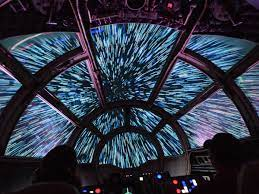
\includegraphics[width=10em]{hyperspace-jump.jpg}}
            \end{center}
        \end{minipage}
        \end{uncoverenv}
        \vskip 0.5em
        \begin{minipage}[t][1cm][t]{0.46\textwidth}
        \begin{center}
            \scalebox{0.7}{
                \vphantom{$\psi = \symbolstack{.one}, \phi = \nilscopestack$}
            }
        \end{center}
        \end{minipage}
        \vskip 0.5em
        \begin{minipage}[c][2cm][c]{0.46\textwidth}
            \begin{center}
            \smaller[1]
            Positional parameter 0 \\
            should have a member named \texttt{one} \\
            which the reference at \textit{a.py:6:16} resolves to. \\
            \end{center}
        \end{minipage}
        \begin{uncoverenv}<2- >
        \phantom{\; $+$ \;}
        \begin{minipage}[c][2cm][c]{0.46\textwidth}
            \begin{center}
            \smaller[1]
            Resolve the \textsf{JUMP} node.
            \end{center}
        \end{minipage}
        \end{uncoverenv}
    \end{center}
\end{frame}


\begin{frame}[fragile]
    \frametitle{The dataflow example}

    \vskip 2em
    \begin{center}
        \begin{minipage}[t]{0.46\textwidth}
            \begin{center}
            \scalebox{0.7}{\partialpath
                {\nilsymbolstack}{\nilscopestack}
                {\node [reference] {one}}
                {\node [exported scope] {A}}
                {\symbolstack{0.one}}{\nilscopestack}}
            \end{center}
        \end{minipage}
        \begin{uncoverenv}<2- >
            \; $+$ \;
        \begin{minipage}[t]{0.46\textwidth}
            \begin{center}
            \scalebox{0.7}{\partialpath
                {\symbolstack{0} \cdot \psi}{\phi}
                {\node [exported scope] {A}}
                {\node [exported scope] {C}}
                {\psi}{\phi}}
            \end{center}
        \end{minipage}
        \end{uncoverenv}
        \vskip 0.5em
        \begin{minipage}[t][1cm][t]{0.46\textwidth}
        \begin{center}
            \scalebox{0.7}{
                \onslide<3>{$\psi = \symbolstack{.one}, \phi = \nilscopestack$}
            }
        \end{center}
        \end{minipage}
        \vskip 0.5em
        \begin{minipage}[c][2cm][c]{0.46\textwidth}
            \begin{center}
            \smaller[1]
            Positional parameter 0 \\
            should have a member named \texttt{one} \\
            which the reference at \textit{a.py:6:16} resolves to. \\
            \end{center}
        \end{minipage}
        \begin{uncoverenv}<2- >
            \; $+$ \;
        \begin{minipage}[c][2cm][c]{0.46\textwidth}
            \begin{center}
            \smaller[1]
            The class \texttt{A} is positional parameter 0 \\
            in the call to \texttt{dataflow.passthrough}. \\
            \end{center}
        \end{minipage}
        \end{uncoverenv}
    \end{center}
\end{frame}


\begin{frame}[fragile]
    \frametitle{The dataflow example}

    \vskip 2em
    \begin{center}
        \begin{minipage}[t]{0.46\textwidth}
            \begin{center}
            \scalebox{0.7}{\partialpath
                {\nilsymbolstack}{\nilscopestack}
                {\node [reference] {one}}
                {\node [exported scope] {C}}
                {\symbolstack{.one}}{\nilscopestack}}
            \end{center}
        \end{minipage}
        \begin{uncoverenv}<2- >
            \; $+$ \;
        \begin{minipage}[t]{0.46\textwidth}
            \begin{center}
            \scalebox{0.7}{\partialpath
                {\symbolstack{.one} \cdot \psi}{\phi}
                {\node [exported scope] {C}}
                {\node [definition] {one}}
                {\psi}{\phi}}
            \end{center}
        \end{minipage}
        \end{uncoverenv}
        \vskip 0.5em
        \begin{minipage}[t][1cm][t]{0.46\textwidth}
        \begin{center}
            \scalebox{0.7}{
                \onslide<3>{$\psi = \nilsymbolstack, \phi = \nilscopestack$}
            }
        \end{center}
        \end{minipage}
        \vskip 0.5em
        \begin{minipage}[c][2cm][c]{0.46\textwidth}
            \begin{center}
            \smaller[1]
            The class \texttt{A} \\
            should have a member named \texttt{one} \\
            which the reference at \textit{a.py:6:16} resolves to. \\
            \end{center}
        \end{minipage}
        \begin{uncoverenv}<2- >
            \; $+$ \;
        \begin{minipage}[c][2cm][c]{0.46\textwidth}
            \begin{center}
            \smaller[1]
            The class \texttt{A} has a class member named \texttt{one} \\
            which is defined at \textit{a.py:4:5}. \\
            \end{center}
        \end{minipage}
        \end{uncoverenv}
    \end{center}
\end{frame}


\begin{frame}[fragile]
    \frametitle{The dataflow example}

    \vskip 2em
    \begin{center}
        \begin{minipage}[t]{0.46\textwidth}
            \begin{center}
            \scalebox{0.7}{\partialpath
                {\nilsymbolstack}{\nilscopestack}
                {\node [reference] {one}}
                {\node [definition] {one}}
                {\nilsymbolstack}{\nilscopestack}}
            \end{center}
        \end{minipage}
        \phantom{\; $+$ \;}
        \begin{minipage}[t]{0.46\textwidth}
            \strut
        \end{minipage}
        \vskip 0.5em
        \begin{minipage}[t][1cm][t]{0.46\textwidth}
        \begin{center}
            \scalebox{0.7}{
                \vphantom{$\psi = \symbolstack{.one}, \phi = \nilscopestack$}
            }
        \end{center}
        \end{minipage}
        \vskip 0.5em
        \begin{minipage}[c][2cm][c]{0.46\textwidth}
            \begin{center}
            \smaller[1]
            The definition at \textit{a.py:4:5} \\
            is what the reference at \\
            \textit{a.py:6:16} resolves to. \\
            \end{center}
        \end{minipage}
        \phantom{\; $+$ \;}
        \begin{minipage}[c][2cm][c]{0.46\textwidth}
            \smaller[1]
            \strut
        \end{minipage}
    \end{center}
\end{frame}


\section{Closing}

\begin{frame}
    \begin{tikzpicture}
        \node (bar) at(0,0) [
            rectangle, anchor=west,
            minimum width=\columnwidth, minimum height=1cm,
            draw=black, thin,
            fill=gray!20,
        ] {};

        \node at(bar.west) [
            rectangle, anchor=west,
            minimum width=0.5\columnwidth, minimum height=1cm,
            draw=black, thin,
            fill=yellow!20,
        ] {};
        \node at(bar.east) [
            rectangle, anchor=east,
            minimum width=0.5\columnwidth, minimum height=1cm,
            draw=black, thin,
            fill=blue!20,
        ] {};

        \node at(bar.west) [
            rectangle, anchor=west, inner xsep=2ex,
            text height=1.5ex, text depth=0.25ex,
            text=black,
        ] {Index};
        \node at(bar.east) [
            rectangle, anchor=east, inner xsep=2ex,
            text height=1.5ex, text depth=0.25ex,
            text=black,
        ] {Query};
    \end{tikzpicture}

    \vskip 1em
    \begin{minipage}{0.49\columnwidth}
    \begin{center}
        Clone changed files \\
        Parse using tree-sitter \\
        Construct stack graph \\
        Find partial paths \\
    \end{center}
    \end{minipage}
    \begin{minipage}{0.49\columnwidth}
    \begin{center}
        Load partial paths lazily \\
        Stitch them together \\
    \end{center}
    \end{minipage}

    \vskip 4em
    \begin{uncoverenv}<2>
    \begin{minipage}{0.49\columnwidth}
    \begin{center}
        p50: 5 sec \\
        p99: 1-2 min \\
    \end{center}
    \end{minipage}
    \begin{minipage}{0.49\columnwidth}
    \begin{center}
        p50: 50ms \\
        p99: 100ms \\
    \end{center}
    \end{minipage}
    \end{uncoverenv}
\end{frame}


\begin{frame}[fragile]
    \frametitle{The \emph{really} hard ones...}

    \highlightdef{one_def}
    \highlightref{one_ref}
    \highlightboth{String}
    \highlightref{length_ref}

    \begin{center}
    \begin{minipage}[t]{9em}
    \begin{minted}[label=dataflow.py]{python}
        def passthrough(x):
            return x

        class A:
            ?\tikzmark{one_def_start}?one?\tikzmark{one_def_end}? = 1

        passthrough(A).?\tikzmark{one_ref_start}?one?\tikzmark{one_ref_end}?
    \end{minted}
    \end{minipage}
    \hspace{3em}
    \begin{minipage}[t]{20em}
    \begin{minted}[label=MyMap.java]{java}
        import java.util.HashMap;

        class MyMap extends HashMap<?\tikzmark{String_start}?String?\tikzmark{String_end}?, String> {
            int firstLength() {
                return this.entrySet().iterator()
                    .next().getKey().?\tikzmark{length_ref_start}?length?\tikzmark{length_ref_end}?();
            }
        }
    \end{minted}
    \end{minipage}
    \end{center}
\end{frame}


\begin{frame}[t]
    \frametitle{Picture credits}
    \begin{tabular}{lp{0.75\textwidth}}
    \picturecredits
    \end{tabular}

    \begin{textblock*}{10mm}(82.5mm,73.5mm)
        \only<2>{
\includegraphics[width=5mm]{repos.png}}
    \end{textblock*}
    \begin{textblock*}{60mm}(90mm,72mm)
        \only<2>{
            \href{https://github.com/github/stack-graphs}{\texttt{github/stack-graphs}} \\
            \href{https://github.com/tree-sitter/tree-sitter-graph}{\texttt{tree-sitter/tree-sitter-graph}}
        }
    \end{textblock*}
\end{frame}


\section{Appendix}

\begin{frame}
    \begin{center}
        \begin{tikzpicture}
            \draw [help lines] (0,0) grid (10,8);

            \node (root)   [root node]       at(1,1)  {};
            \node (s0)     [anon scope]      at(2,1)  {};
            \node (sB)     [named scope]     at(3,1)  {B};
            \node (s7)     [exported scope]  at(4,1)  {7};
            \node (A)      [definition]      at(1,2)  {\PopSymbol{A}};

            \node (a)      [definition]  [right=of A] {\PopSymbol{a}};
            \node (A2)     [pop]         [above=of A] {\PopSymbol{A\textsubscript{2}}};
            \node (main2)  [pop]         [right=of A2] {\PopSymbol{\_\_main\_\_\textsubscript{2}}};
            \node (bar)    [pop]         [right=of main2] {\PopScopedSymbol{A\textsubscript{3}}};

            \node (A3)     [reference]  [above=of A2] {\PushSymbol{A}};
            \node (a3)     [reference]  [right=of A3] {\PushSymbol{a}};
            \node (A4)     [push]       [above=of A3] {\PushSymbol{A\textsubscript{4}}};
            \node (main4)  [push]       [right=of A4] {\PushSymbol{\_\_main\_\_\textsubscript{4}}};
            \node (foo)    [push]       [right=of main4] {\PushScopedSymbol{A\textsubscript{3}}{7}};

            % edges
            \path [-Stealth]
              (root) edge (A)
              (A) edge (a)
                  edge (A2)
              (a) edge (main2)
              ;
        \end{tikzpicture}
    \end{center}
\end{frame}


\section{Producing stack graphs}

\begin{frame}
    \frametitle{Are we done?}
    \begin{itemize}
        \item \textcolor<2,4>{lightgray}{Different languages have different name binding rules.}
        \item \textcolor<2,4>{lightgray}{Some of those rules can be quite complex.}
        \item \textcolor<3,4>{lightgray}{The result might depend on intermediate files.}
        \item \textcolor<2,3>{lightgray}{We don't want to require manual per-repo configuration.}
        \item \textcolor<3,4>{lightgray}{We need incremental processing to handle our scale.}
    \end{itemize}
\end{frame}


\begin{frame}
    \begin{textblock*}{160mm}(0mm,-16mm)
        \picturecredit{Dave Lawler}{Good Morning}{CC-BY-2.0}{https://flic.kr/p/WYowT7}
        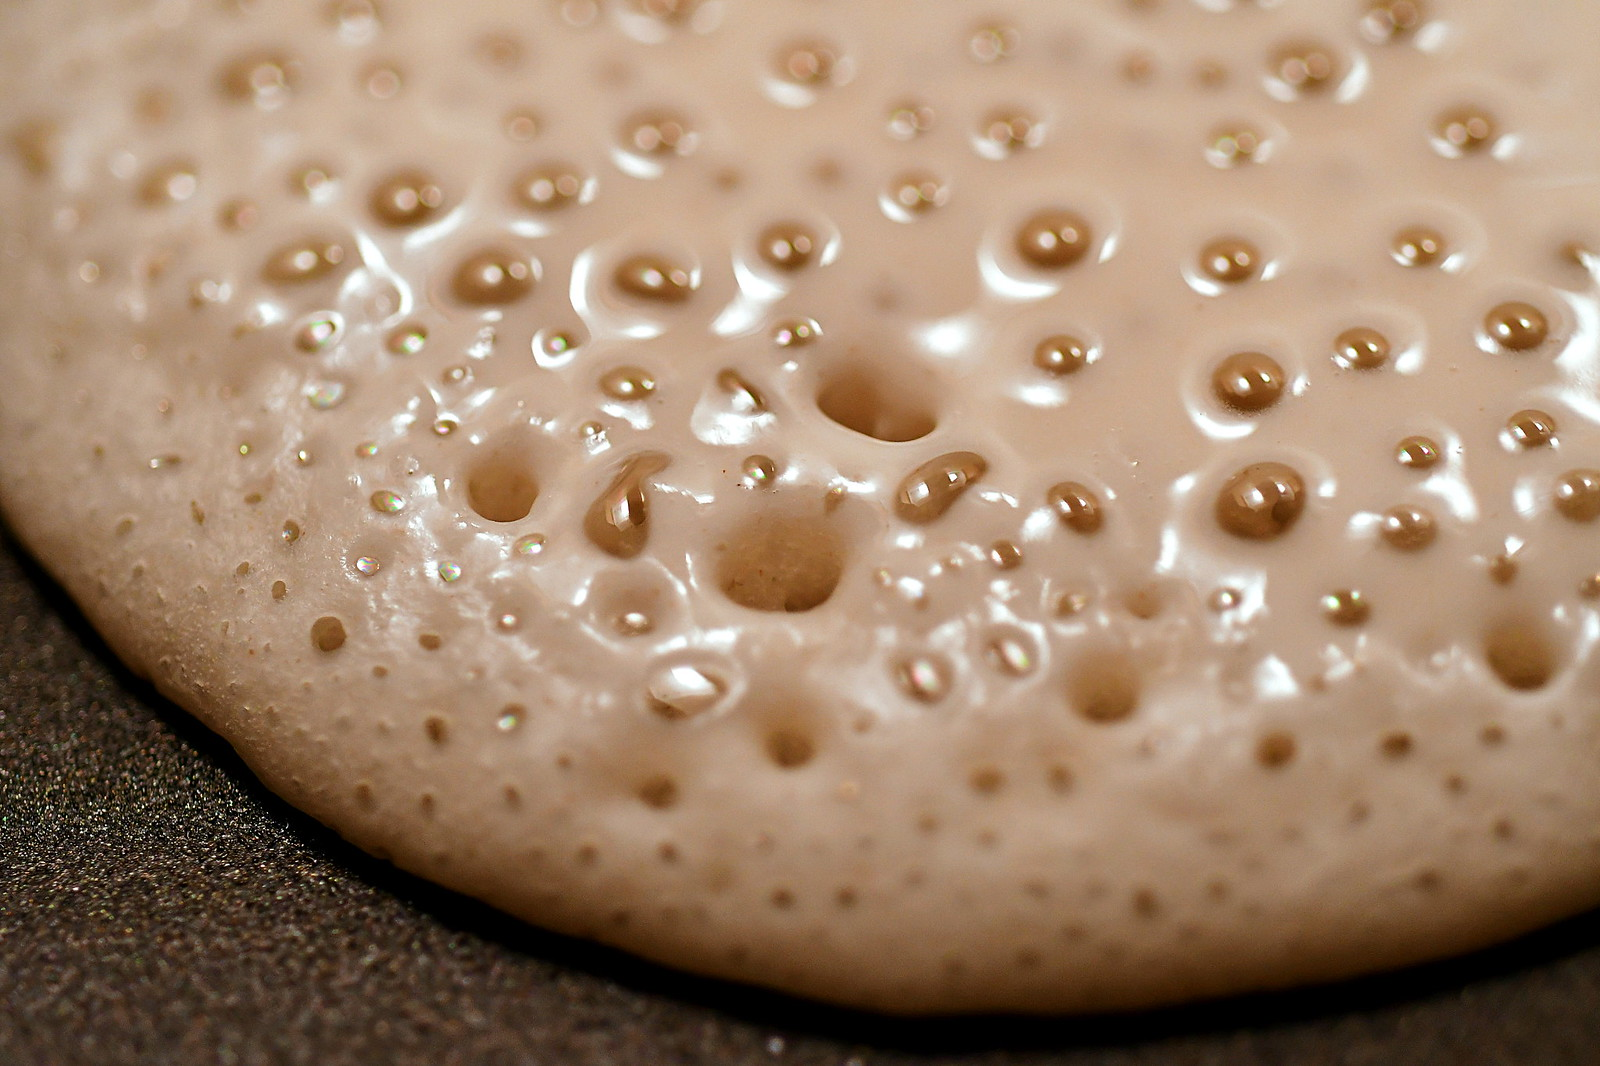
\includegraphics[width=160mm]{pancake-stove.jpg}
    \end{textblock*}
    \shadowedtitle{8mm}{80mm}{Making stack graphs}
\end{frame}


\begin{frame}
    \begin{textblock*}{160mm}(0mm,-16mm)
        \picturecredit{Tony Guyton}{Treehouse Point}{CC-BY-2.0}{https://flic.kr/p/rRrT5F}
        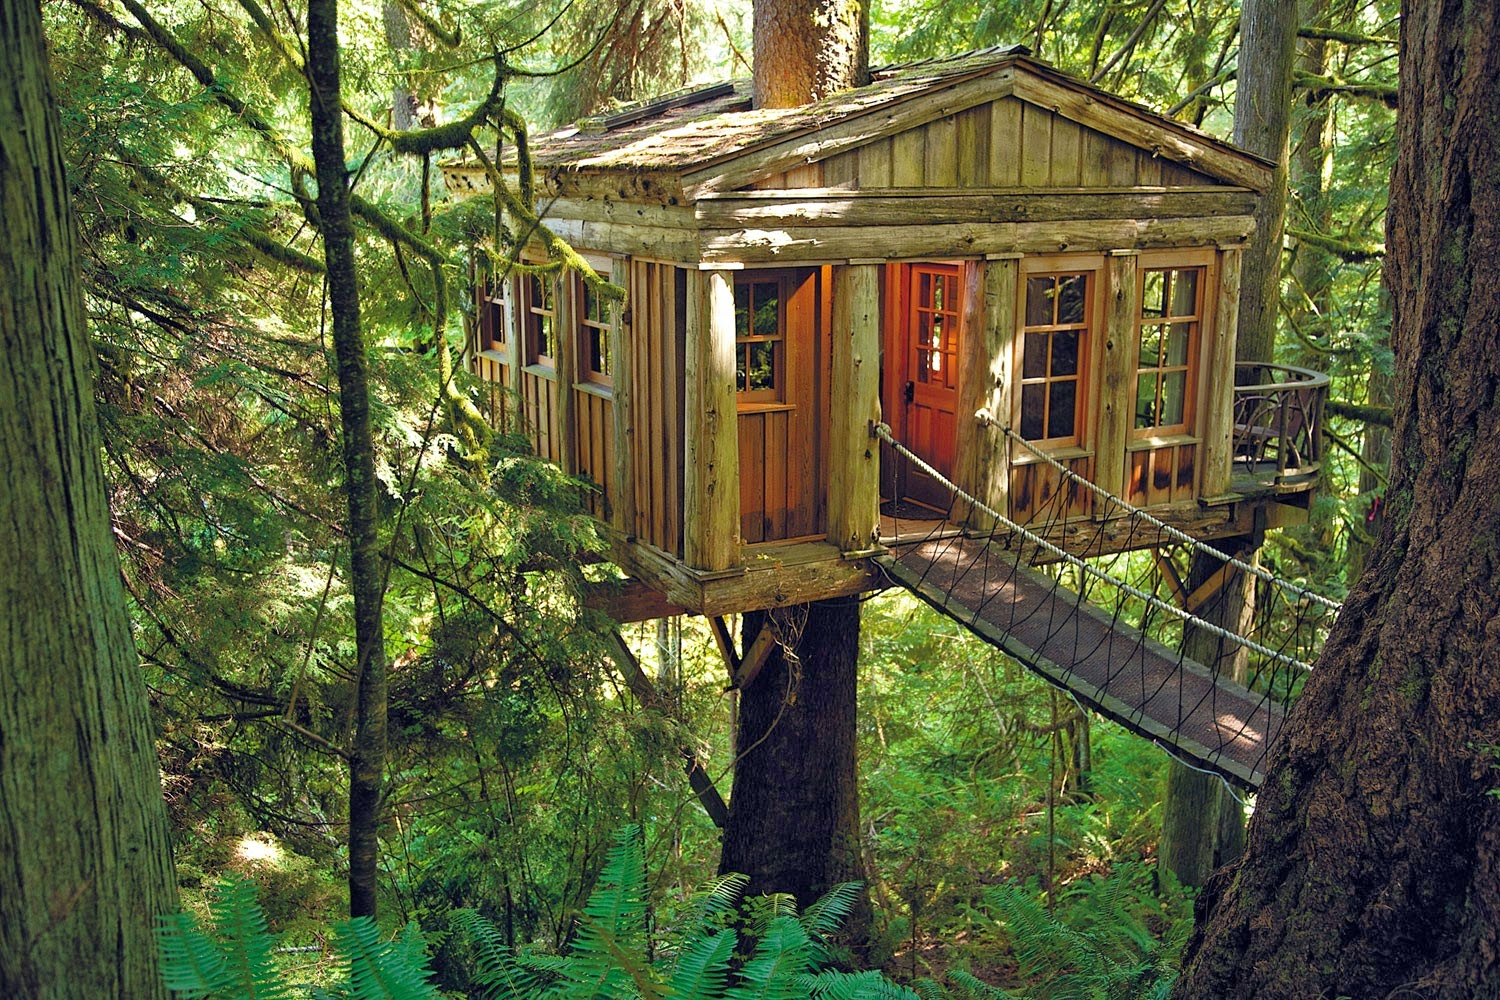
\includegraphics[width=160mm]{treehouse.jpg}
    \end{textblock*}
    \shadowedtitle{80mm - 0.5\titlewidth}{75mm}{\href{https://tree-sitter.github.io/}{tree-sitter}}
\end{frame}


\begin{frame}[fragile]
    \frametitle{tree-sitter}
    \begin{center}
    \begin{minipage}{0.75\textwidth}
    \begin{minipage}{9em}
    \begin{minted}[label=stove.py]{python}
        def bake():
            pass

        def broil():
            pass

        def saute():
            pass

        broil()
    \end{minted}
    \end{minipage}
    \end{minipage}
    \end{center}
\end{frame}


\begin{frame}[fragile]
    \frametitle{tree-sitter}

    \uncover<3-4>{\highlightparse{blue!25}{func}}
    \uncover<3-4>{\highlightcapture{blue!25}{func}}
    \uncover<4>  {\highlightparse{yellow!50}{name}}
    \uncover<4>  {\highlightcapture{yellow!50}{name}}

    \begin{center}
    \begin{minipage}{0.75\textwidth}
    \begin{minipage}{12em}
    \begin{minted}[fontsize={\smaller[4]},frame=none]{text}
        (module [0, 0] - [10, 0]
          (function_definition [0, 0] - [1, 8]
            name: (identifier [0, 4] - [0, 8])
            parameters: (parameters [0, 8] - [0, 10])
            body: (block [1, 4] - [1, 8]
              (pass_statement [1, 4] - [1, 8])))
          ?\tikzmark{func_start}?(function_definition [3, 0] - [4, 8]
            name: ?\tikzmark{name_start}?(identifier [3, 4] - [3, 9])?\tikzmark{name_end}?
            parameters: (parameters [3, 9] - [3, 11])
            body: (block [4, 4] - [4, 8]
              (pass_statement [4, 4] - [4, 8])))     ?\tikzmark{func_end}?
          (function_definition [6, 0] - [7, 8]
            name: (identifier [6, 4] - [6, 9])
            parameters: (parameters [6, 9] - [6, 11])
            body: (block [7, 4] - [7, 8]
              (pass_statement [7, 4] - [7, 8])))
          (expression_statement [9, 0] - [9, 7]
            (call [9, 0] - [9, 7]
              function: (identifier [9, 0] - [9, 5])
              arguments: (argument_list [9, 5] - [9, 7]))))
    \end{minted}
    \end{minipage}
    \hspace{1em}
    \begin{minipage}{15em}
    \begin{uncoverenv}<2- >
    \begin{minted}[fontsize=\scriptsize,frame=none]{text}
        (function_definition
          name: (identifier) ?\tikzmark{name_capture_start}?@name?\tikzmark{name_capture_end}?) ?\tikzmark{func_capture_start}?@function?\tikzmark{func_capture_end}?
    \end{minted}
    \end{uncoverenv}

    \begin{uncoverenv}<5- >
    \begin{minted}[fontsize=\scriptsize,frame=none]{text}
        {
            node @function.def
            attr (@function.def) kind = "definition"
            attr (@function.def) symbol = @name

            edge @function.containing_scope -> @function.def
        }
    \end{minted}
    \end{uncoverenv}
    \begin{uncoverenv}<6>
    \begin{center}
    \begin{tikzpicture}
        \node (s) [anon scope] {};
        \node (d) [definition] [right=of s] {\textit{@name}};
        \path [-Stealth] (s) edge (d);
    \end{tikzpicture}
    \end{center}
    \end{uncoverenv}
    \end{minipage}

    \end{minipage}
    \end{center}
\end{frame}

\begin{frame}
    \begin{textblock*}{10mm}(10mm,13mm)
        
\includegraphics[width=8mm]{icons/graph.jpg}
    \end{textblock*}
    \begin{textblock*}{60mm}(20mm,10mm)
        \href{https://github.com/github/stack-graphs}{\texttt{github/stack-graphs}} \\
        \href{https://github.com/tree-sitter/tree-sitter}{\texttt{tree-sitter/tree-sitter}} \\
        \href{https://github.com/tree-sitter/tree-sitter-graph}{\texttt{tree-sitter/tree-sitter-graph}} \\
    \end{textblock*}

    \begin{textblock*}{10mm}(68mm,29.5mm)
        \only<2>{
\includegraphics[width=5mm]{languages/python.png}}
    \end{textblock*}
    \begin{textblock*}{60mm}(75mm,30mm)
        \only<2>{\href{https://github.com/tree-sitter/tree-sitter-python}{\texttt{tree-sitter/tree-sitter-python}}}
    \end{textblock*}

    \begin{textblock*}{10mm}(68mm,36.25mm)
        \only<2>{
\includegraphics[width=5mm]{languages/javascript.png}}
    \end{textblock*}
    \begin{textblock*}{70mm}(75mm,37mm)
        \only<2>{\href{https://github.com/tree-sitter/tree-sitter-javascript}{\texttt{tree-sitter/tree-sitter-javascript}}}
    \end{textblock*}

    \begin{textblock*}{10mm}(68mm,43.5mm)
        \only<2>{
\includegraphics[width=5mm]{languages/rust.png}}
    \end{textblock*}
    \begin{textblock*}{60mm}(75mm,44mm)
        \only<2>{\href{https://github.com/tree-sitter/tree-sitter-rust}{\texttt{tree-sitter/tree-sitter-rust}}}
    \end{textblock*}

    \begin{textblock*}{10mm}(68mm,50.5mm)
        \only<2>{
\includegraphics[width=5mm]{languages/ruby.png}}
    \end{textblock*}
    \begin{textblock*}{60mm}(75mm,51mm)
        \only<2>{\href{https://github.com/tree-sitter/tree-sitter-ruby}{\texttt{tree-sitter/tree-sitter-ruby}}}
    \end{textblock*}

    \begin{textblock*}{10mm}(68mm,57mm)
        \only<2>{
\includegraphics[width=5mm]{languages/elixir.png}}
    \end{textblock*}
    \begin{textblock*}{60mm}(75mm,58mm)
        \only<2>{\href{https://github.com/elixir-lang/tree-sitter-elixir}{\texttt{elixir-lang/tree-sitter-elixir}}}
    \end{textblock*}

    \begin{textblock*}{10mm}(68mm,64.75mm)
        \only<2>{
\includegraphics[width=5mm]{languages/r.png}}
    \end{textblock*}
    \begin{textblock*}{60mm}(75mm,65mm)
        \only<2>{\href{https://github.com/r-lib/tree-sitter-r}{\texttt{r-lib/tree-sitter-r}}}
    \end{textblock*}

    \begin{textblock*}{10mm}(100mm,71mm)
        \only<2>{\vdots}
    \end{textblock*}
\end{frame}


\begin{frame}[fragile]
    \frametitle{Extras}

    \highlightdef{broil1}
    \highlightdef{broil2}

    \begin{center}

    \begin{minipage}{9em}
    \begin{minted}[label={stove.rs}]{rust}
        fn ?\tikzmark{broil1_start}?broil?\tikzmark{broil1_end}?() {}

        fn ?\tikzmark{broil2_start}?broil?\tikzmark{broil2_end}?() {}

        fn saute() {}
    \end{minted}
    \end{minipage}
    \hspace{2em}
    \begin{tikzpicture}[baseline={(current bounding box.center)}]
        \node (root)       [root node]                              {};
        \node (stove)      [definition]  [left=of root]             {\PopSymbol{stove}};
        \node (dot)        [pop]         [left=of stove]            {\PopSymbol{::}};

        \node (s)          [anon scope]  [above=2\scopegap of dot]  {};

        \setwidestsymbol{\PopSymbol{broil}}
        \node (broil2 def) [definition]  [left=of s]                {\sized{\PopSymbol{broil}}};
        \node (saute def)  [definition]  [below=of broil2 def]      {\sized{\PopSymbol{saute}}};
        \node (broil1 def) [definition]  [above=of broil2 def]      {\sized{\PopSymbol{broil}}};

        \path [-Stealth]
          (root)      edge (stove)
          (stove)     edge (dot)
          (dot)       edge (s)
          (s)         edge (saute def)
                      edge (broil2 def)
                      edge (broil1 def)
          ;
    \end{tikzpicture}

    \end{center}
\end{frame}

\end{document}
